%TEX-template borrowed from https://github.com/idlouhy/wonsole/blob/master/report/src/report.tex

\documentclass[12pt,a4paper,oneside]{report}

\usepackage[section] {placeins}

\usepackage[english]{babel}
\usepackage[utf8]{inputenc}
\usepackage[T1]{fontenc}
\usepackage{float}

\selectlanguage{english}

\usepackage{graphicx}
\usepackage{tabu}
\usepackage{booktabs}
\usepackage{wrapfig}
\usepackage{pbox}
\usepackage{pgfplots}
\usepackage{pgfplotstable}
\usepackage{longtable}
\usepackage{pdfpages}
\usepackage{mathtools}
\usepackage{graphicx}
\usepackage{subcaption}
\usepackage{csquotes}
\usepackage{rotating}

\usepackage{nameref}
\usepackage{fullpage}
\usepackage{verbatim}
\usepackage{url}
\usepackage{cite}
\usepackage{caption}
\usepackage{float}
\usepackage{color}
\usepackage{hyperref}

% Library for syntax highlighting
\usepackage{minted}

\usepgfplotslibrary{dateplot}

\usemintedstyle[glsl]{colorful}
\usemintedstyle[c]{colorful}
\usemintedstyle[cpp]{colorful}

\setlength{\parindent}{0.0in}
\setlength{\parskip}{1.5ex}

\setlength{\fboxsep}{0pt}
\setlength{\fboxrule}{1pt}

\fontfamily{ptm}\selectfont

\usepackage{hyperref}
\hypersetup{
    bookmarks=true,
    unicode=true,
    pdftoolbar=true,
    pdfmenubar=true,
    pdffitwindow=false,
    pdfstartview={FitH},
    pdftitle={OpenGL Labs TDT4195},
    pdfauthor={Bart van Blokland},
    pdfsubject={Introduction to OpenGL},
    pdfkeywords={ntnu} {OpenGL} {GLSL} {TDT4195},
    pdfnewwindow=true,
    colorlinks=false,
    linkcolor=blue,
    citecolor=blue,
    filecolor=blue,
    urlcolor=blue
}


\bibliographystyle{ieeetr}

\begin{document}

%TITLE

\thispagestyle{empty}

\begin{center}
    {\Huge\textbf{A Hitchhiker's Guide to OpenGL}} \\  

    \vspace{1cm}

    {\large Bart van Blokland}\\

    \vspace{18cm}

	{\large Department of Computer and Information Science, NTNU}\\
	\vspace{1cm}
    {\large Revision 4.2}\\ 
\end{center}

\newpage

\setcounter{tocdepth}{1}
\tableofcontents
\clearpage

% CHAPTERS

\chapter{A bird's eye view of OpenGL}

\section{What is OpenGL?}

At a very high level, OpenGL is a library which allows rendering of geometric shapes. This process is nowadays as good as ubiquitously accelerated by specialised hardware, commonly referred to as a GPU (Graphics Processing Unit).

You should think of OpenGL as a pipeline. You insert data on one end, and a little while later an image pops out at the other end. 

This pipeline is not a ``One Size Fits All'', however. There are a large number of settings which you are able to change which affect the final image produced. Moreover, specific components of the pipeline called ``Shaders'' are missing by default, and must be defined in order to complete the pipeline.

The number of possible ways in which the pipeline can be configured is immense. The sheer number of features can be very overwhelming when initially jumping into OpenGL. For this reason, this guide will only focus on the basics of rendering geometry and using shaders.

On the next page you can see a (somewhat simplified) overview over what the OpenGL pipeline conceptually looks like. The two mandatory Shaders have been marked with dashed lines, while ``fixed functionality'' automatically performed on the graphics card is indicated with grey boxes.

\centerline{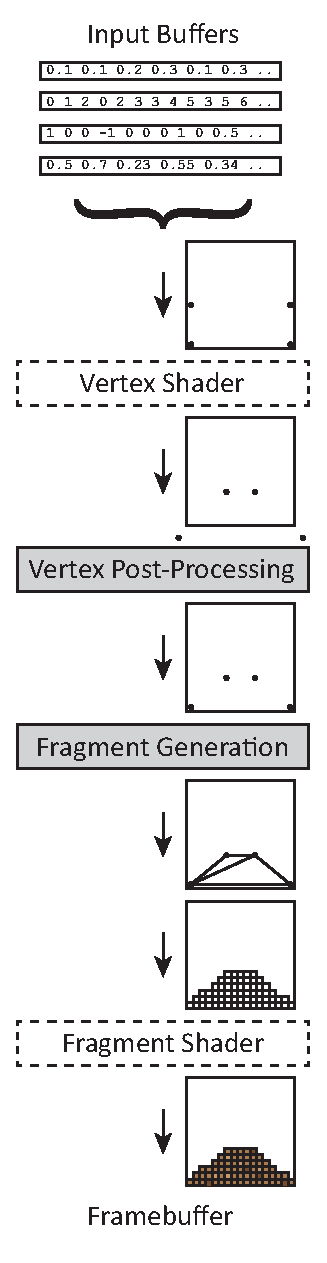
\includegraphics[scale=1.1]{images/pipeline-overview.eps}}

Let's go over each of the indicated stages in the order in which they are listed. Please keep in mind this description disregards a lot of details. 

Rendering an object starts with defining said object. OpenGL needs to know a geometric definition of the object before anything can be drawn. Objects are defined as a list of vertices (points), which can be connected into shapes such as lines or triangles. This input data resides in input buffers, which are created and filled before they can be drawn.

Once you have created and filled your input buffers, you can invoke the geometry processing pipeline by issuing so-called ``draw calls''. A draw call is a kind of transaction in which you indicate which content from your input buffers you would like to draw using the current pipeline configuration. The graphics driver will subsequently invoke the processing pipeline on the GPU and process the specified input.

The first stage of the pipeline is the execution of the vertex shader. The vertex shader is a small program which is executed in its entirety once for every single vertex rendered. Each time it is executed, it takes a vertex as input and outputs a modified vertex. The idea here is that a model can be moved around a scene or animated by applying a series of transformations on each vertex. For 3D scenes, all vertices in a scene must be transformed every frame.

Once all vertices have been processed by an instance of the vertex shader, some additional processing is necessary. Amongst others, clipping is performed as well as the viewport transform. We'll return to clipping specifically a little later, because it's a key part of understanding what you're doing when drawing objects in OpenGL.

Now that the vertex positions are known, vertices can be connected together to form shapes, most commonly triangles. These shapes are in turn rasterised into pixels. The diagram specifically shows what this looks like for triangles. The vertex post-processing and rasterisation is usually all done in hardware on the graphics processor. You don't have to do any of that yourself.

The second mandatory shader in the pipeline is the ``fragment shader''. It takes a rasterised pixel as input, and is responsible for assigning a colour to it. It is executed once for each rasterised pixel. The word ``fragment'' in OpenGL is used to describe a rasterised pixel which is being drawn, but may not necessarily end up being shown in the final image. This can for example happen if another piece of geometry is drawn over the fragment at a later time while rendering the frame. 

The final output is written to a so-called framebuffer. The framebuffer is either directly or indirectly (in case of a windowing system) sent to a monitor to be displayed.

\section{The ClipBox}

As mentioned previously, I'd like to put special emphasis on the clipping process, because it is vital for understanding what is going on when rendering geometry.

Clipping is essentially the process of throwing away all geometry which exceeds the bounds of the screen. If a shape only partially sticks out of the clipping volume, it is cut down exactly to fit within the clipping volume. Clipping also ensures that objects behind the camera are not visible in the rendered image. 

In OpenGL, the clipping volume is defined to be a cube around the origin, which ranges between the values of -1 and 1 along each major axis.

The vertex shader is responsible for compressing the entire contents of your scene into this little 2x2x2 cube, no matter how large the dimensions of your scene are. Anything outside of it will not appear on screen.

Moreover, there is one particular side of this clipbox which has been defined to be the side from which you as a viewer look into the box at the scene you're rendering. The OpenGL standard defines this side to the one on the side of the \emph{negative z-axis} looking into the \emph{positive} direction. 

Here is a visualisation of the clipbox, with the aforementioned viewing side highlighted:

\vspace{0.5cm}
\centerline{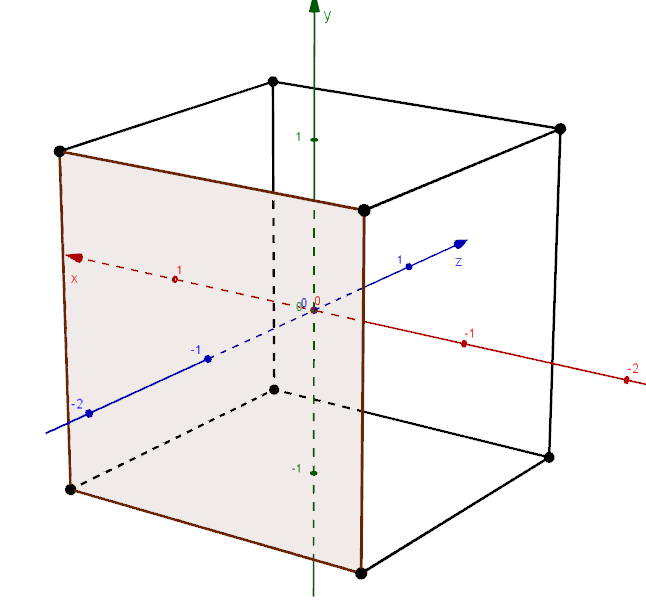
\includegraphics[scale=0.7]{images/clipbox_corrected.png}}
\newpage
\section{OpenGL functions}

The design of OpenGL at its core is that of a state machine. When starting your application, you create a so-called ``OpenGL context''. After doing so, you issue commands to the context by calling OpenGL functions. These functions cause state within the context to change, hence the state machine designation. 

You should think of this state as all data and settings necessary for configuring the OpenGL pipeline. You set up the pipeline in such a way that it will draw the object you want in the way you would like it to. When ready, you issue a draw call and the object is rendered by the pipeline.

Using this style of API may be somewhat counter-intuitive if you've never interacted with such an interface before. However, in practice main difference with more ``conventional'' libraries is that you don't create any data structures or objects yourself. Instead, you give commands to OpenGL which causes the objects to be created for you inside the context. You can subsequently use other functions to modify these objects.

As you will see in later chapters of this guide, setting up various kinds of OpenGL state often implies calling a series of functions in a specific order, rather than issuing a single command. 

OpenGL functions have a very distinct format, making them very easy to distinguish. Here's an example:

\begin{minted}{c}
void glUniform4f(int location, float v0, float v1, float v2, float v3);
\end{minted}

What this function does is not very relevant at this point. Instead, notice the ``gl'' prefix, which is common to all OpenGL functions. 

In some cases a function also allows you to specify the datatype and the number of operands if multiple values are allowed. These functions contain type modifiers at the end of their name, such as the one shown above. In this case, the ``4'' indicates you'd like to pass 4 values, and the ``f'' indicates you're passing in values with a floating point datatype. 

Similarly, the function \mintinline{c}{glUniform3i()} indicates you'll pass in 3 integer values.

Looking up an OpenGL function in the documentation will show you all possible combinations of type modifiers of that particular function.

I want to make one note on the functions listed in this guide. The OpenGL documentation commonly lists rather cryptic data types for each of the parameters. For the sake of being able to understand them, I changed them to those you will be most commonly calling these functions with. If you want the official specifications, I recommend using the official online documentation pages.
\chapter{Introduction to Drawing}

\section{Defining Geometry}

OpenGL can in principle only draw 3 kinds of shapes, known as ``primitives''; triangles, lines and points.


\includegraphics[scale=0.15]{images/openGL_primitives.eps}

Of these three, the triangle is the one that's most commonly used in practice. Primitives combined into shapes are commonly referred to as \emph{geometry}.

Why only three basic shapes? What about rectangles, circles, ellipses, spheres, and so on? 

There are two reasons for this. First, as you will see in the lectures rasterising and rendering triangles is very easy and can therefore be performed very cheaply on the graphics card and accelerated in hardware. Second, you can approximate all the shapes I listed using triangles anyway. 

As mentioned previously, defining a shape in OpenGL consists of defining a list of vertices, which are subsequently combined into primitives that can be rendered. We will now take a look at how these vertex lists can be created, filled with geometry, and prepared to be inserted into the rendering pipeline.

\subsection{Specifying vertices}

The central component in defining a renderable model is an object known as a \emph{Vertex Array Object} (VAO). Its main purpose is linking the contents of input buffers to vertex shader inputs.

\begin{center}
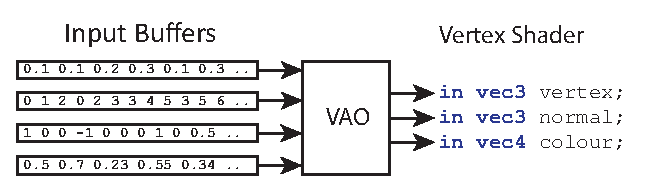
\includegraphics{images/vao-overview.eps}
\end{center}

The illustration above should give a general idea on what is going on. On the left hand side, there are input buffers containing geometry which you'd like to draw. On the right hand side are shown some inputs to the vertex shader, which are defined in the shader source code (don't worry about understanding these variables; we'll deal with them in detail later). 

The link which a VAO represents is the one between data contained inside an input buffer, and an input to the vertex shader. You are responsible for creating these links, and it's easiest to do so while creating the input buffers.

It's common to use a separate VAO for every model in your scene. What the word model \emph{means} in this context depends on what you define it to be. For instance, if you want to render a car, the car's body could be stored in one VAO and the tires in a separate one. It's also possible to store the entire model in a single VAO.

The input buffers used to store input data are known as \emph{Vertex Buffer Objects} (VBO's). The contents of a VBO are generally stored on the memory bank (VRAM) of your graphics card. You therefore have to explicitly transfer data to it before you can use it to draw things.

The sole purpose of VBO's is to hold data. They do not know how their contents are formatted, what their contents represent, nor where their contents are supposed to be used. All of that information is held by the Vertex Array Object.

We'll now look at how you can create your very own Vertex Array Object, followed by how to define and fill a Vertex Buffer Object, and set both up for rendering.

\subsubsection{Creating and setting up a Vertex Array Object}

The first step is to create a new Vertex Array Object using:

\begin{minted}{c}
void glGenVertexArrays(int count, unsigned int* arrayIDs);
\end{minted}

The arrayIDs parameter requires a pointer to a location where the generated array ID(s) can be stored. You are responsible for allocating enough space for these. If not you can cause data corruption or even crashes. For instance, trying to allocate 5 VAO's while passing in an integer array containing 3 entries may cause data corruption on your program stack.

However, the function is relatively easy to use when only allocating a single VAO. Simply create an empty unsigned int on the previous line (\mintinline{cpp}{unsigned int array = 0;}), and pass a reference to it into the function using the \& operator (\mintinline{c}{&array}). The ID of the VAO will be stored in \mintinline{c}{array} afterwards. For simplicity I recommend only generating one VAO at a time unless you really know what you're doing.

The first thing to note here is that you don't actually get a Vertex Array \emph{Object}, but instead the \emph{ID} of the generated VAO. As such you don't actually get to modify the object directly. Instead you use the ID to refer to the array whenever you want to do anything with it. You modify it through OpenGL function calls. 

This is common to the design of all data structures in OpenGL: you only get references instead of complete data structures.

If we want to link Vertex Buffer Objects to shader inputs using the Vertex Array Object, we have to ensure any configuration values are set \emph{while the VAO is active}. You can imagine this process to be like opening a file; in order to add some lines of text (the VBO's) to a text file (the VAO), you first have to open it. As OpenGL is a state machine, this ``file'' will remain open until another one is opened in its place. This process is referred to as \emph{binding}.

Like object references, the concept of binding objects is also used in many other places throughout the OpenGL API. 

The function for binding a vertex array object is defined as follows:

\begin{minted}{c}
void glBindVertexArray(unsigned int vertexArrayID);
\end{minted}

\subsubsection{Creating buffers}

Now that we have created and bound a VAO, we can proceed with defining a Vertex Buffer Object to hold the geometry data of our model. In order to set up a VBO, fill it with data, and create a connection to a shader input in the VAO, there is a particular sequence of functions you need to call. We'll be taking a look at these functions below.

The first step is to create the Vertex Buffer Object. This function works identically to the one used for creating VAO's:

\begin{minted}{c}
void glGenBuffers(int count, unsigned int* bufferIDs);
\end{minted}

Note that even though the buffer is meant to hold data, you don't need to specify the size of your buffer at this point. OpenGL will perform these allocations behind the scenes as you fill or append data to your buffer.

\subsubsection{Binding buffers}

Like Vertex Array Objects, Vertex Buffer Objects are also required to be \emph{bound} before they can be modified, and only one can be bound at a time. 

The function for binding a buffer is:

\begin{minted}{c}
void glBindBuffer(enum target, unsigned int bufferID);
\end{minted}

The target parameter specifies which kind of buffer you would like to bind your buffer as. Most of these types are advanced uses that are not relevant for this course. You'll therefore usually want to pass in \mintinline{c}{GL_ARRAY_BUFFER} here.

The bufferID parameter is the ID of the buffer you would like to work with. This should be the buffer ID you generated using \mintinline{c}{glGenBuffers()}.

It is possible to ``unbind'' a VBO by binding a buffer with an ID of 0. However, it is not something that ought to be done in practice for two reasons. First, any subsequent time a buffer is going to be modified, it will have to be bound first anyway. Second, binding and unbinding buffers may incur additional overhead on the OpenGL driver implementation side.

\subsubsection{Filling buffers}

Now that we have created and bound our buffer, we can fill it with data. This of course requires that you already have some geometry data to fill it with. A general method for doing so is to allocate an array of floats (although other data types will work too):
\begin{minted}{c}
                //   x    y    z    x    y    z    x    y    z  .. and so on
float vertices[] = {1.0, 3.0, 2.0, 5.0, 4.0, 3.0, 2.0, 6.0, 3.0};
\end{minted}

In practice, this data usually originates from a separate file. 

Once you have your float array ready to go, you can use the \mintinline{c}{glBufferData()} function to transfer the data to the GPU:

\begin{minted}{c}
void glBufferData(enum target, size_t size, void* data, enum usage);
\end{minted}

The target parameter has to match the target parameter you supplied in the \mintinline{c}{glBindBuffer()} call.

The size parameter is the size of your data array in bytes. You'll probably need to use the \mintinline{c}{sizeof(/* data type */)} function here, which returns the number of bytes a particular datatype occupies in memory. Note that \mintinline{c}{sizeof()} takes in a datatype as its parameter, such as \mintinline{c}{float} or \mintinline{c}{int}. 

It is in some cases possible to pass the array into the \mintinline{c}{sizeof()} function directly to get the number of bytes occupied by the array's contents in memory.

For instance:

\begin{minted}{c}
int someArray[] = {1, 2, 3};
printf("The size of someArray in bytes is \%i.\n", sizeof(someArray));
// Prints: "The size of someArray in bytes is 12."
\end{minted}

However, whenever an array is passed as a parameter into another function, it is quietly converted into a pointer. This even happens when the function parameter has the array type. As a pointer only represents a memory address, the array dimensions information is lost. As such calling sizeof() on the array variable will give you the size of the pointer (usually 8 bytes on a 64 bit system), rather than the total size of the array.

It may therefore be beneficial to pass in the length of the array into the function as a separate parameter, so this confusing behaviour can be avoided altogether. In that case, multiply the length of the array with the size of the datatype of that array (e.g. \mintinline{c}{arrayLength * sizeof(float)}) to get the size of the array in bytes.

Next is the data parameter, which (surprise surprise) contains a pointer to the data which should be copied to the GPU. Note that the type of this parameter is a \mintinline{c}{void} pointer. A \mintinline{c}{void} pointer in C means that you can supply a pointer to any data type you want. So for instance \mintinline{c}{float*} or \mintinline{c}{int*} are both valid parameter types here.

The usage parameter provides a hint to the purpose of the data you're supplying. Based on this parameter, the OpenGL implementation may perform optimisations to a greater or lesser degree, if at all. It does not restrict how you can use the buffer. 

For basic rendering of models it's best to use \mintinline{c}{GL_STATIC_DRAW} here. The \mintinline{c}{STATIC} component indicates that the contents of the buffer are not expected to change often, if at all. The alternatives for \mintinline{c}{STATIC} are \mintinline{c}{DYNAMIC} and \mintinline{c}{STREAM}, which are intended for increasing modification rates to the buffer.

The \mintinline{c}{DRAW} component indicates that the contents of the buffer are intended for rendering geometry. The alternatives are more advanced uses outside the scope of this guide.

\subsubsection{Format Specification}

You may have noticed from the \mintinline{c}{glBufferData()} function specification that there was no requirement for defining the format of your buffer. OpenGL does not know whether you passed in floats or integers, nor does it know whether you specified x, y and z coordinates, or only x and y coordinates.

For this reason we have to set a \emph{Vertex Attribute Pointer}. A Vertex Attribute is a term used to refer to an input of the vertex shader. A Vertex Attribute Pointer specifies where the vertex shader can obtain the data for a particular vertex attribute and how it is formatted.

Here's the function for setting the Vertex Attribute Pointer:

\begin{minted}{c}
void glVertexAttribPointer(
    unsigned int index, 
    int size, 
    enum type, 
    bool normalised, 
    size_t stride, 
    void* pointer
);
\end{minted}

Even more parameters than \mintinline{c}{glBufferData()}! Let's go over them.

The index parameter specifies the index of the vertex attribute pointer you would like to set. Don't worry if that doesn't make sense right now, we'll come back to it in the section about Shaders. In a nutshell you give each Vertex Attribute in the vertex shader a number, and use the same number in this function to connect the VBO to the Vertex Attribute.

This is a number you can make up yourself, as long as it is between 0 and the OpenGL constant \mintinline{c}{GL_MAX_VERTEX_ATTRIBS}, and you use the same IDs for the same Vertex Attribute both in OpenGL function calls as well as your Shader source code. 

Note that the values of OpenGL constants need to be queried. You can find out the value of the constant by using:

\begin{minted}{c}
int maxVertexAttribs;
glGetIntegerv(GL_MAX_VERTEX_ATTRIBS, &maxVertexAttribs);
printf("GL_MAX_VERTEX_ATTRIBS: %i\n", maxVertexAttribs);
\end{minted}

On modern machines, this value is almost always 16.

The size parameter can either be 1, 2, 3 or 4. It defines the number of components per \emph{entry} in the buffer. For instance, only specifying x and y coordinates per vertex means that \mintinline{c}{size} should be 2. If you specify x, y and z coordinates, \mintinline{c}{size} is 3, and so on.

\mintinline{c}{Type} defines the data type of the values in the buffer. This should match the type of values you passed in with the \mintinline{c}{glBufferData()} call. Here's some of the possible data types you can pass in here:

\begin{itemize}
	\item \mintinline{c}{GL_BYTE}
	\item \mintinline{c}{GL_UNSIGNED_BYTE}
	\item \mintinline{c}{GL_SHORT}
	\item \mintinline{c}{GL_UNSIGNED_SHORT}
	\item \mintinline{c}{GL_INT}
	\item \mintinline{c}{GL_UNSIGNED_INT}
	\item \mintinline{c}{GL_FLOAT}
\end{itemize}

Performance tip: you should always choose the smallest possible data type possible that is acceptable for your data. For instance, if you have a buffer of positive integers whose values never exceed 255, you can make indices of the type \mintinline{c}{GL_UNSIGNED_BYTE}. Doing this can significantly reduce the memory bandwidth requirements of the graphics card, increasing performance.

Next up is the \mintinline{c}{normalised} parameter. It defines whether OpenGL should normalise the values in your buffer. In most cases you'll want to pass \mintinline{c}{GL_FALSE} here. 

The \mintinline{c}{stride} parameter defines the number of bytes between each \emph{entry} in the buffer. This may sound strange at first; if a buffer only contains coordinates, can't you just calculate these from the other parameters? The thing is that if you want, a single Vertex Buffer Object can contain multiple Vertex Attributes. For instance, you can pack both vertex coordinates and texture coordinates \footnote{In a nutshell, textures are images that can be mapped on to triangles. Texture Coordinates tell OpenGL what part of such an image to project on a given triangle. Since textures are (usually) two-dimensional objects, you can use two coordinates to define locations on the texture itself. The ``u'' and ``v'' names by which each axis is often referred to is the origin of the other common name for textures; UV maps.} in the same buffer:

\centerline{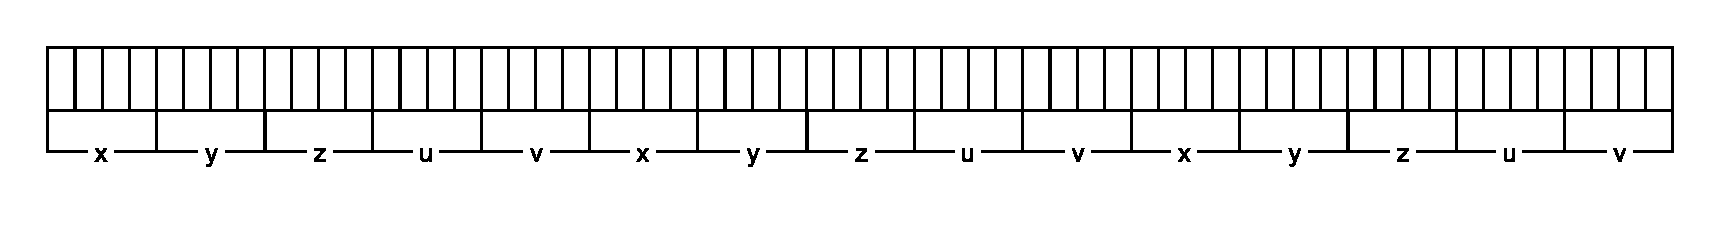
\includegraphics[scale=0.6]{images/openGL_interleaved_buffer.eps}}

In this case, the buffer contains 3 floating point coordinate components (x, y, and z) of 4 bytes each, as well as 2 texture coordinates of 4 bytes each. The number of bytes from the first byte of an x coordinate to the next is 20 bytes. This is known as the \emph{stride}. 

If your buffer only contains a single entry type, you can pass in 0 here, and OpenGL will deduce the stride for you based upon the values of other parameters. However, when multiple entry types are present such as in the example shown above, you're responsible for determining the proper stride yourself.

Finally, the \mintinline{c}{pointer} parameter defines the number of bytes until the first value in the buffer. Using the example from the buffer shown above, the x, y and z coordinates start at index 0, while the texture coordinates start at byte $3 \cdot 4 = 12$. If you only have a single entry type in your buffer, this parameter is usually 0.

\subsubsection{Enabling the Vertex Attributes}

Finally, we need to enable the Vertex Buffer Objects that should serve as input to the rendering pipeline. Inputs can be enabled with: 

\begin{minted}{c}
void glEnableVertexAttribArray(unsigned int index);
\end{minted}

The index parameter should correspond to the index you passed into the \mintinline{c}{glVertexAttribPointer()} while setting up the VAO. You need to call \mintinline{c}{glEnableVertexAttribArray()} once for every Vertex Attribute you would like to use as input for rendering.

Calling \mintinline{c}{glVertexAttribPointer()} and \mintinline{c}{glEnableVertexAttribArray()} ensures the Vertex Attributes are linked to shader inputs when you issue a draw call. 

And that's it! Your Vertex Attribute is now active within the VAO, ready to be used. However, there's one more step before we can draw its contents.

\subsection{The index buffer}

We now have a buffer which defines the coordinates of a number of vertices. However, we did not specify any information about how these are supposed to be combined into primitives. We can do this through the use of a special buffer called an ``index buffer''. 

You might wonder why we have to specify an additional buffer to combine vertices into primitives instead of just using the vertices in the order they are defined in your VBO? To answer this, let's take a look at a cube made up of triangles:\\

\centerline{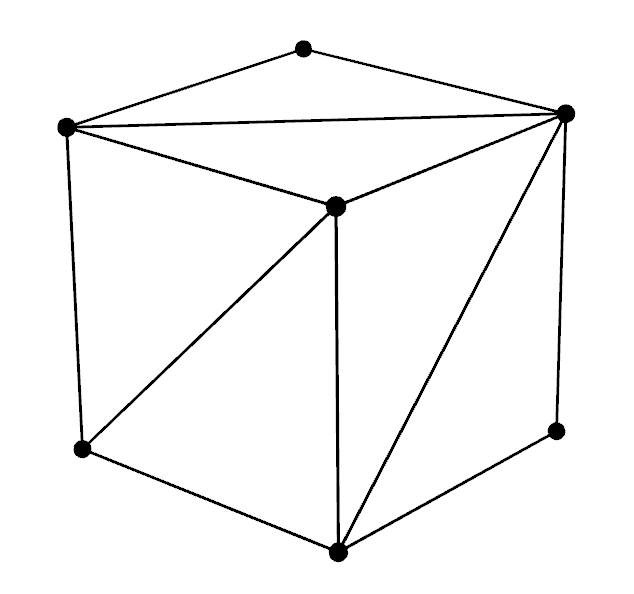
\includegraphics[scale=0.3]{images/cube.png}}

Notice how most vertices are part of multiple triangles. The center one is even part of 4 of them. 3D surfaces tend to be ``watertight'' in order to appear convincing on the rendered image. As this requires using the same vertices several times over for different triangles, it makes sense to only define the vertices once, and combine them together by referring to their \emph{index} in the VBO. If executed well, you can save quite a bit of memory usage. 

This process is comparable to the ``connect the dots'' puzzles, where a set of vertices with associated indices are defined which can be connected into a shape. The only difference here is that vertices with arbitrary indices can be combined into points, lines, triangles or otherwise. An example of such a puzzle is shown below \footnote{Original image by whitney waller, red lines added - connect-the-dots, CC BY-SA 2.0, https://commons.wikimedia.org/w/index.php?curid=45762476}:

\centerline{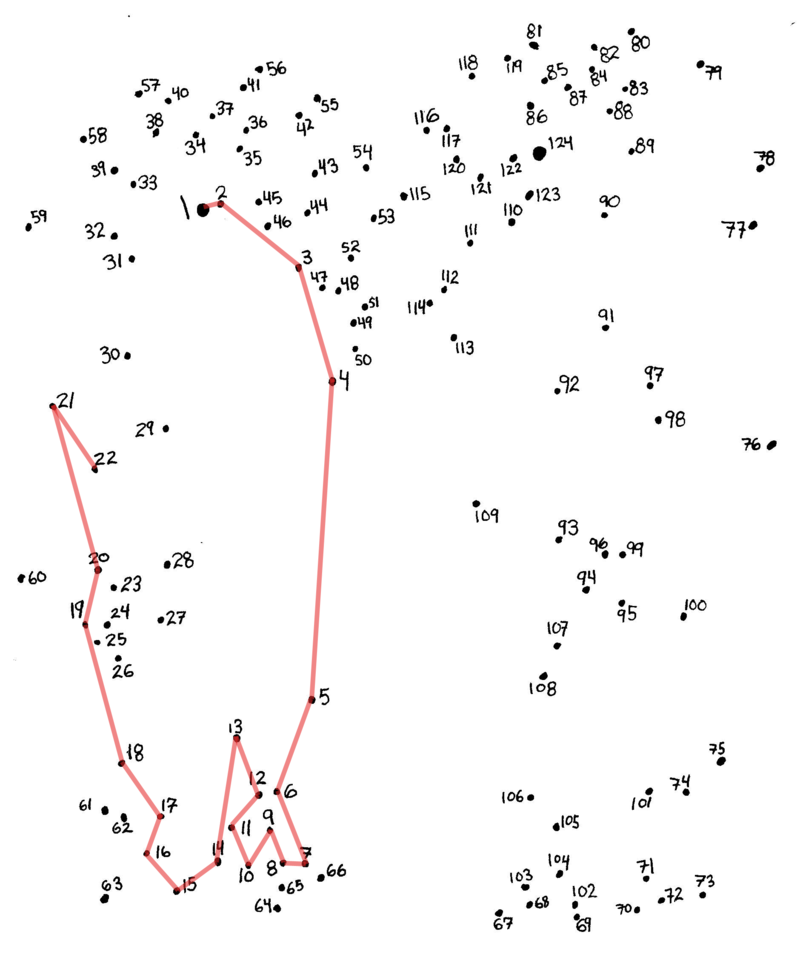
\includegraphics[scale=0.3]{images/Connect_the_dots_puzzle_(partially_solved).png}}

Fortunately, the mechanism for creating and filling an index buffer is very similar to the way we set up VBO's. I'll therefore only outline the differences here.

First, you generate another buffer using \mintinline{c}{glGenBuffers()}.

Next, you bind the generated buffer with as target \mintinline{c}{GL_ELEMENT_ARRAY_BUFFER}, as opposed to \mintinline{c}{GL_ARRAY_BUFFER}. The index buffer has a special ``status'' within the Vertex Array Object and thus has a separate buffer type.

Now we can fill the buffer with indices. They should be unsigned integers, unsigned shorts or unsigned chars (bytes). Just like with the VBO's you should create an array of these. The index of the vertices you defined in your VBO start counting at 0.

Finally, we call \mintinline{c}{glBufferData()} to copy the integer array into the index buffer. Note that the target should in this case also be \mintinline{c}{GL_ELEMENT_ARRAY_BUFFER}.

And we're done! We're now ready to draw our Vertex Array Object :)

Unlike the VBO's, you don't need to call \mintinline{c}{glVertexAttribPointer()} to set up your index buffer.

\newpage
\subsubsection{Visualised Example}

\makebox[\textwidth]{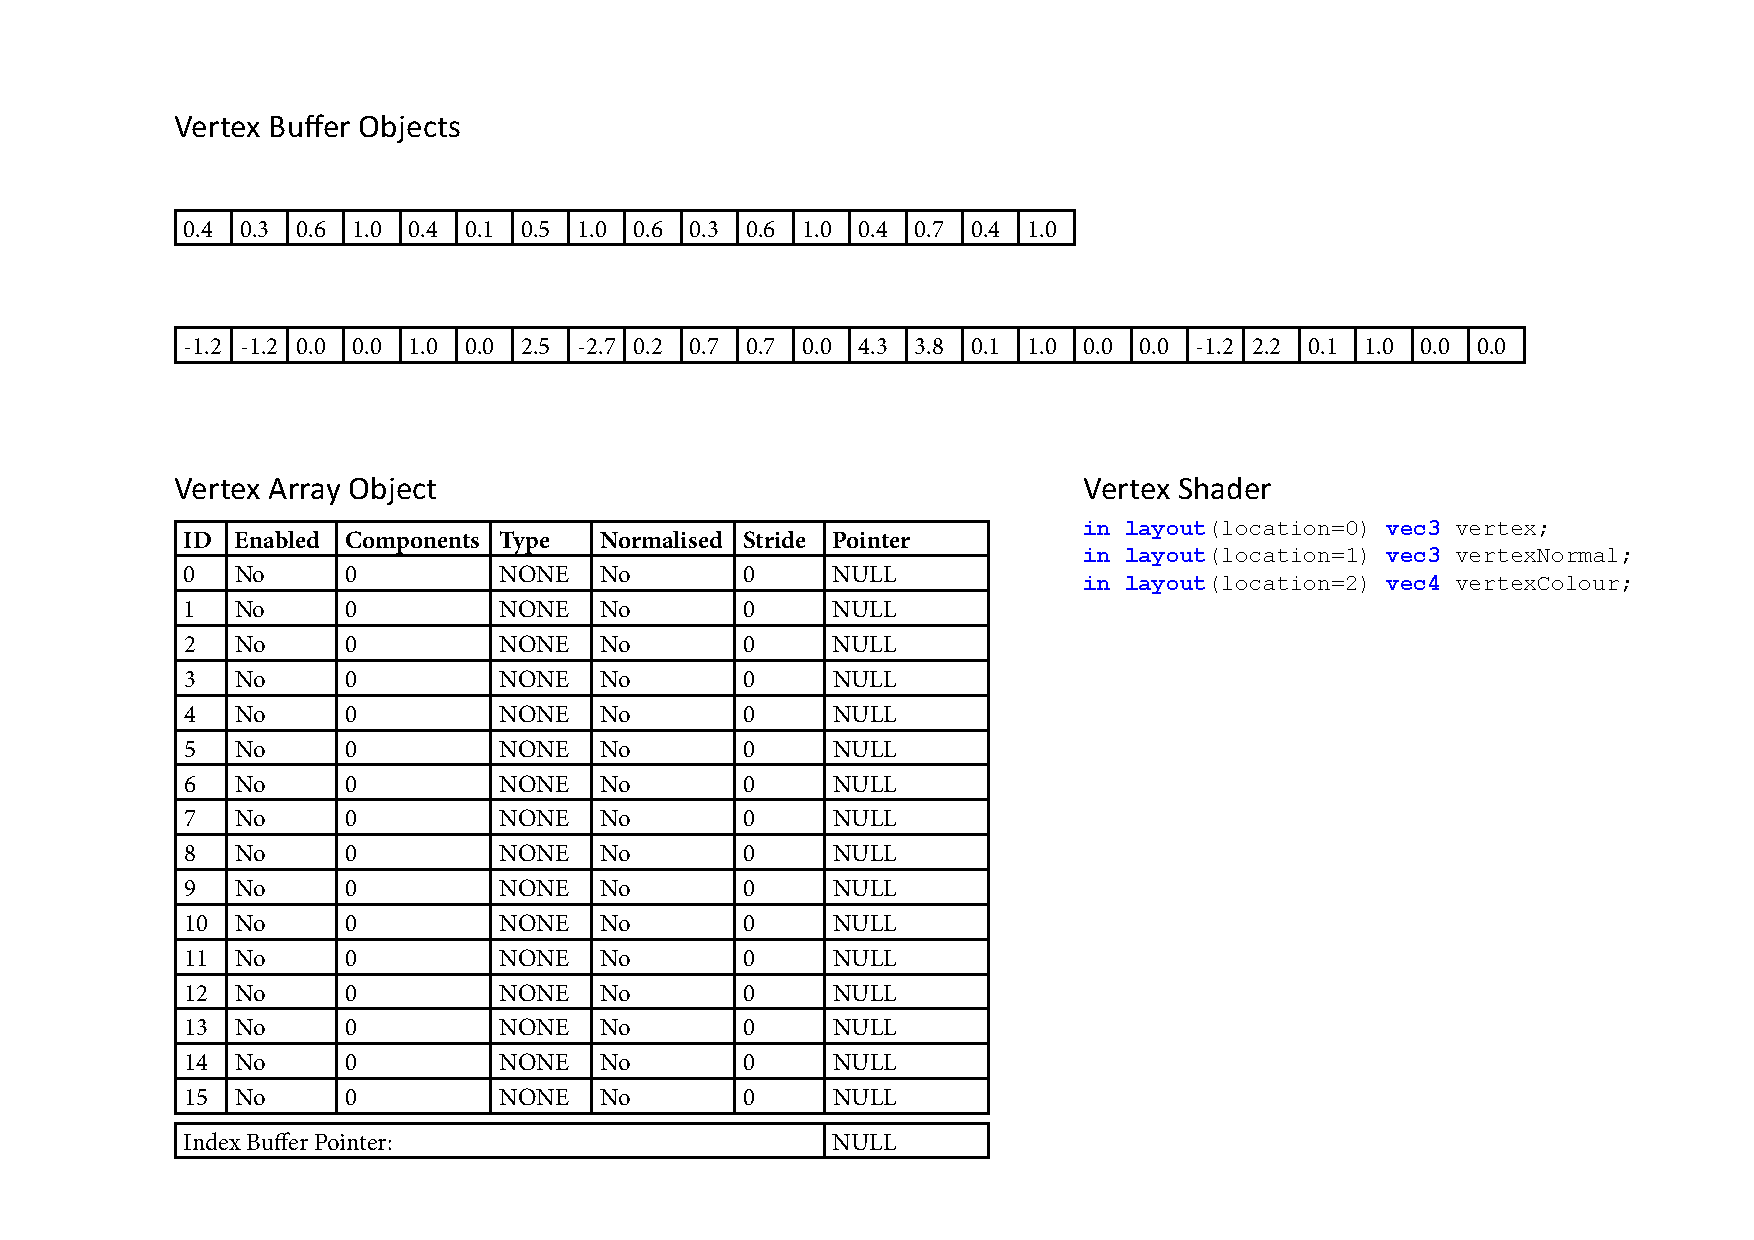
\includegraphics[width=210mm]{images/VAO_initial.pdf}}

Now that we've seen the functions needed to create and fill VBO's and set up a VAO, let's pause for a moment and take a closer look at a practical example to see what effect calling each function in the setup process has.

We'll start with a situation where we've already created some VBO's containing input for the rendering pipeline. We've also created an empty vertex array object. Note that in practice, a VAO really is nothing more than a table containing an entry for each possible vertex attribute index, plus a pointer to an index buffer. This table is created by OpenGL internally, so it's not something you create yourself. 

Finally, there is some shader code on the right hand side of the diagram. We'll come back to shaders in detail in a later chapter, but what's relevant here is that the \mintinline{glsl}{in} keyword declares an input variable to the shader. Additionally, the \mintinline{glsl}{layout(location=0)} qualifier refers to a vertex attribute index, and \mintinline{glsl}{vec3} and \mintinline{glsl}{vec4} are floating point vectors of 3 and 4 elements, respectively. 

\makebox[\textwidth]{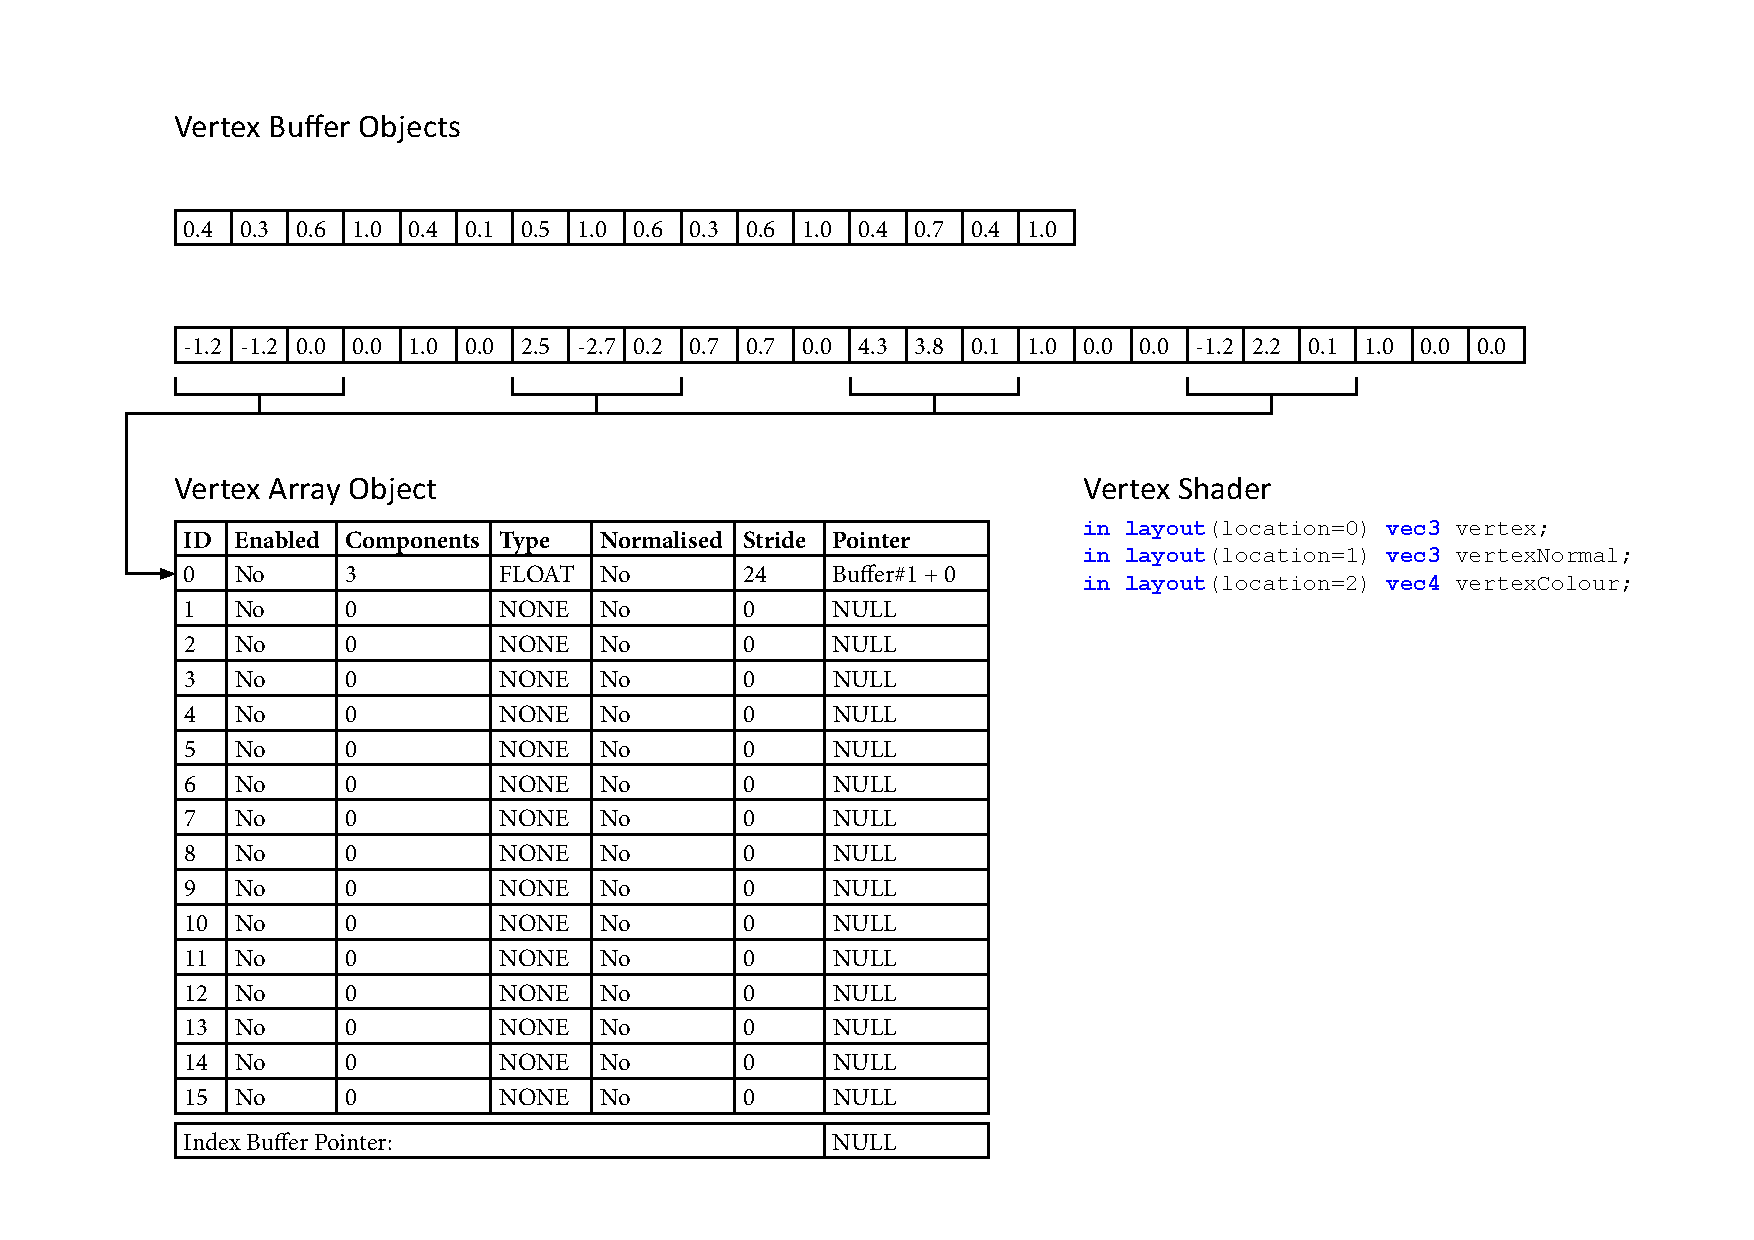
\includegraphics[width=210mm]{images/VAO_vert.pdf}}

As mentioned earlier, after having created and filled a VBO, we can use the function \mintinline{c}{glVertexAttribPointer()} to specify the format of our input buffer. 

As indicated, the number of components (or values) per entry in the buffer is 3. Also their datatype (float) is stored in the table.

Note that the buffer contains definitions of vertices as well as vertex surface normal vectors (used in lighting calculations, amongst other things). This affects the stride of the vertex attribute. Since the buffer only contains floating point numbers, each element in the entire buffer uses 4 bytes of space. There are 6 elements from one entry to the next, which means $4 \cdot 6 = 24$ bytes of stride between each entry.

The requirement for having the source VBO bound when calling \mintinline{c}{glVertexAttribPointer()} is due to a pointer being stored to the first byte of the vertex attribute contents. 

\newpage

\makebox[\textwidth]{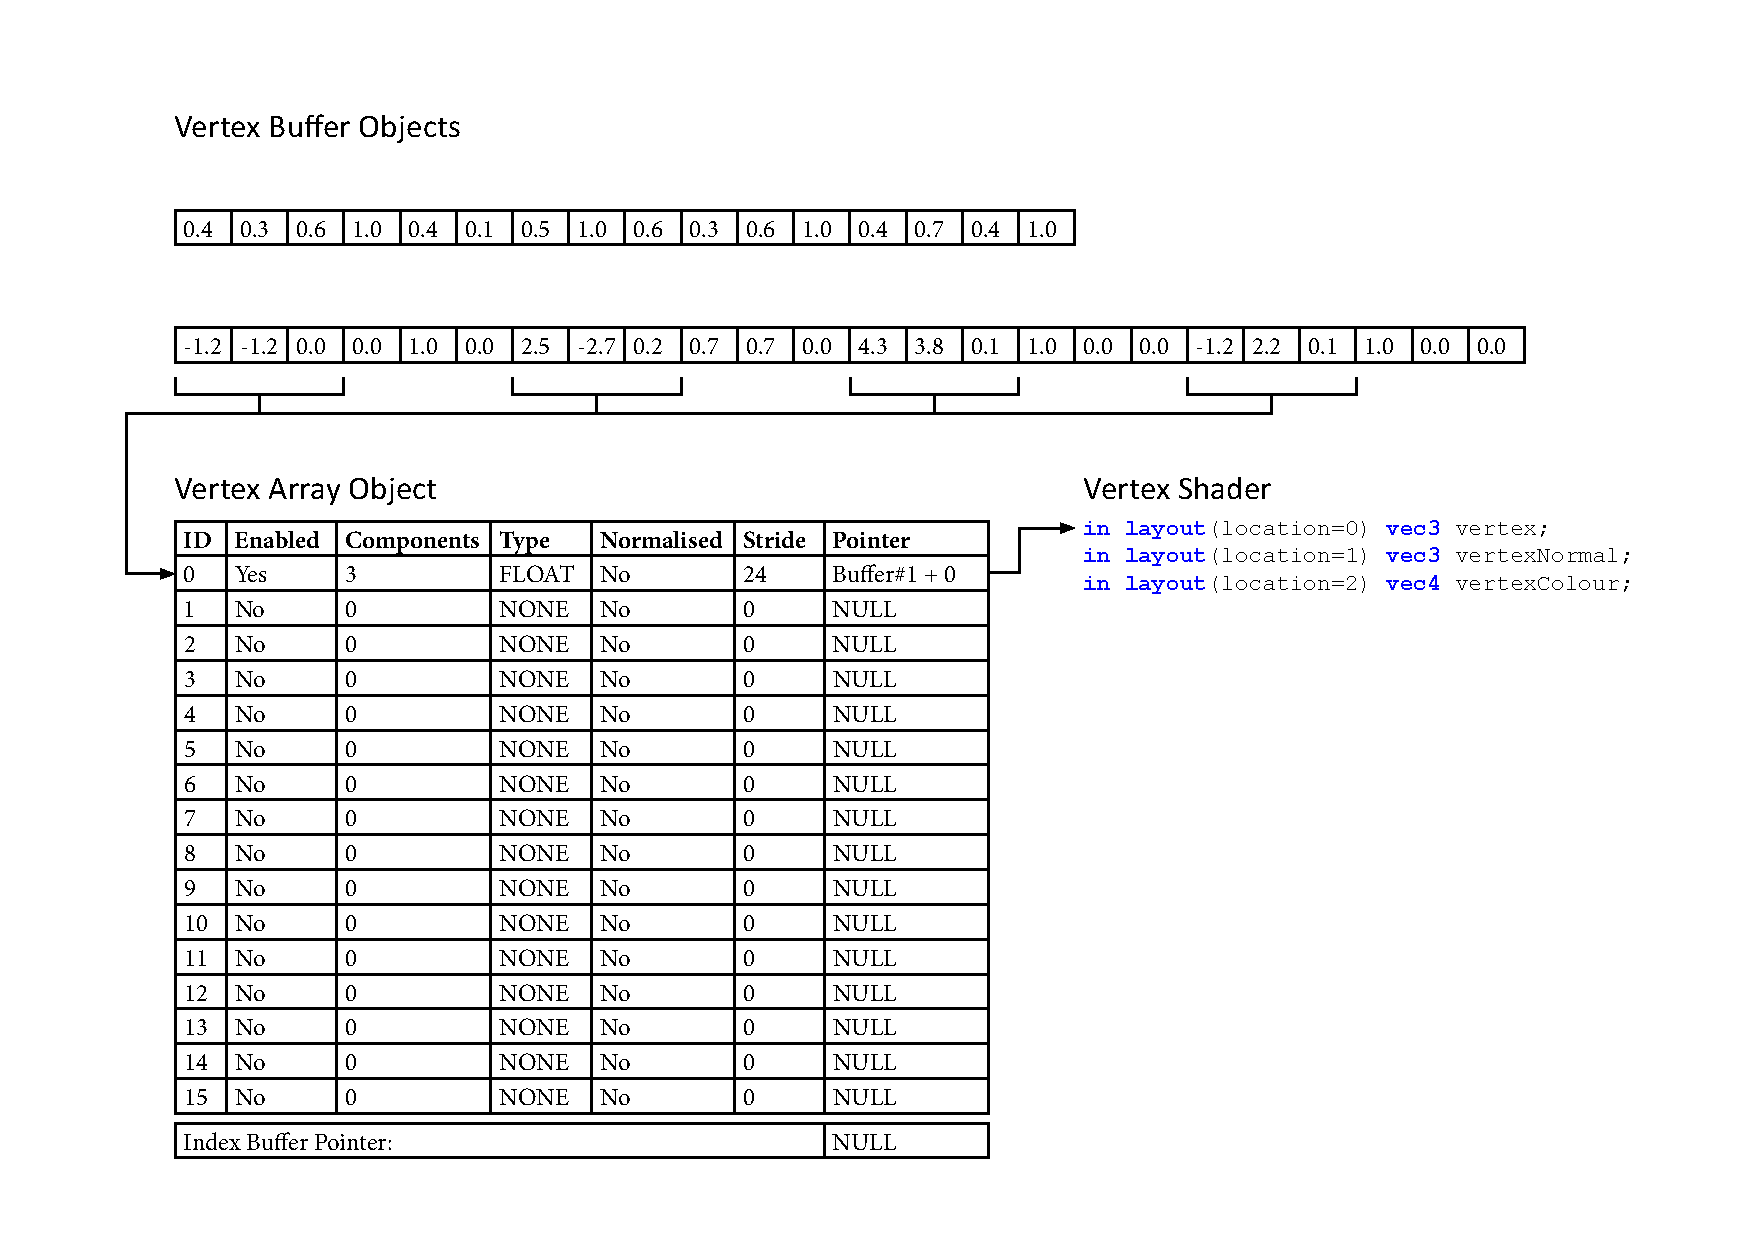
\includegraphics[width=210mm]{images/VAO_vert_enabled.pdf}}

Remember the need to call the \mintinline{c}{glEnableVertexAttribArray()} function? Here you can see its result. It simply marks a vertex attribute in the vertex array object as enabled, thereby completing the connection from the VAO to a shader input. Since entries are disabled by default, you're responsible to enabling those which you need for rendering.

Notice the effective result thus far: input data which can be located in arbitrary buffers with arbitrary sizes and formatting can be sent as input to arbitrary shaders. 

\newpage

\makebox[\textwidth]{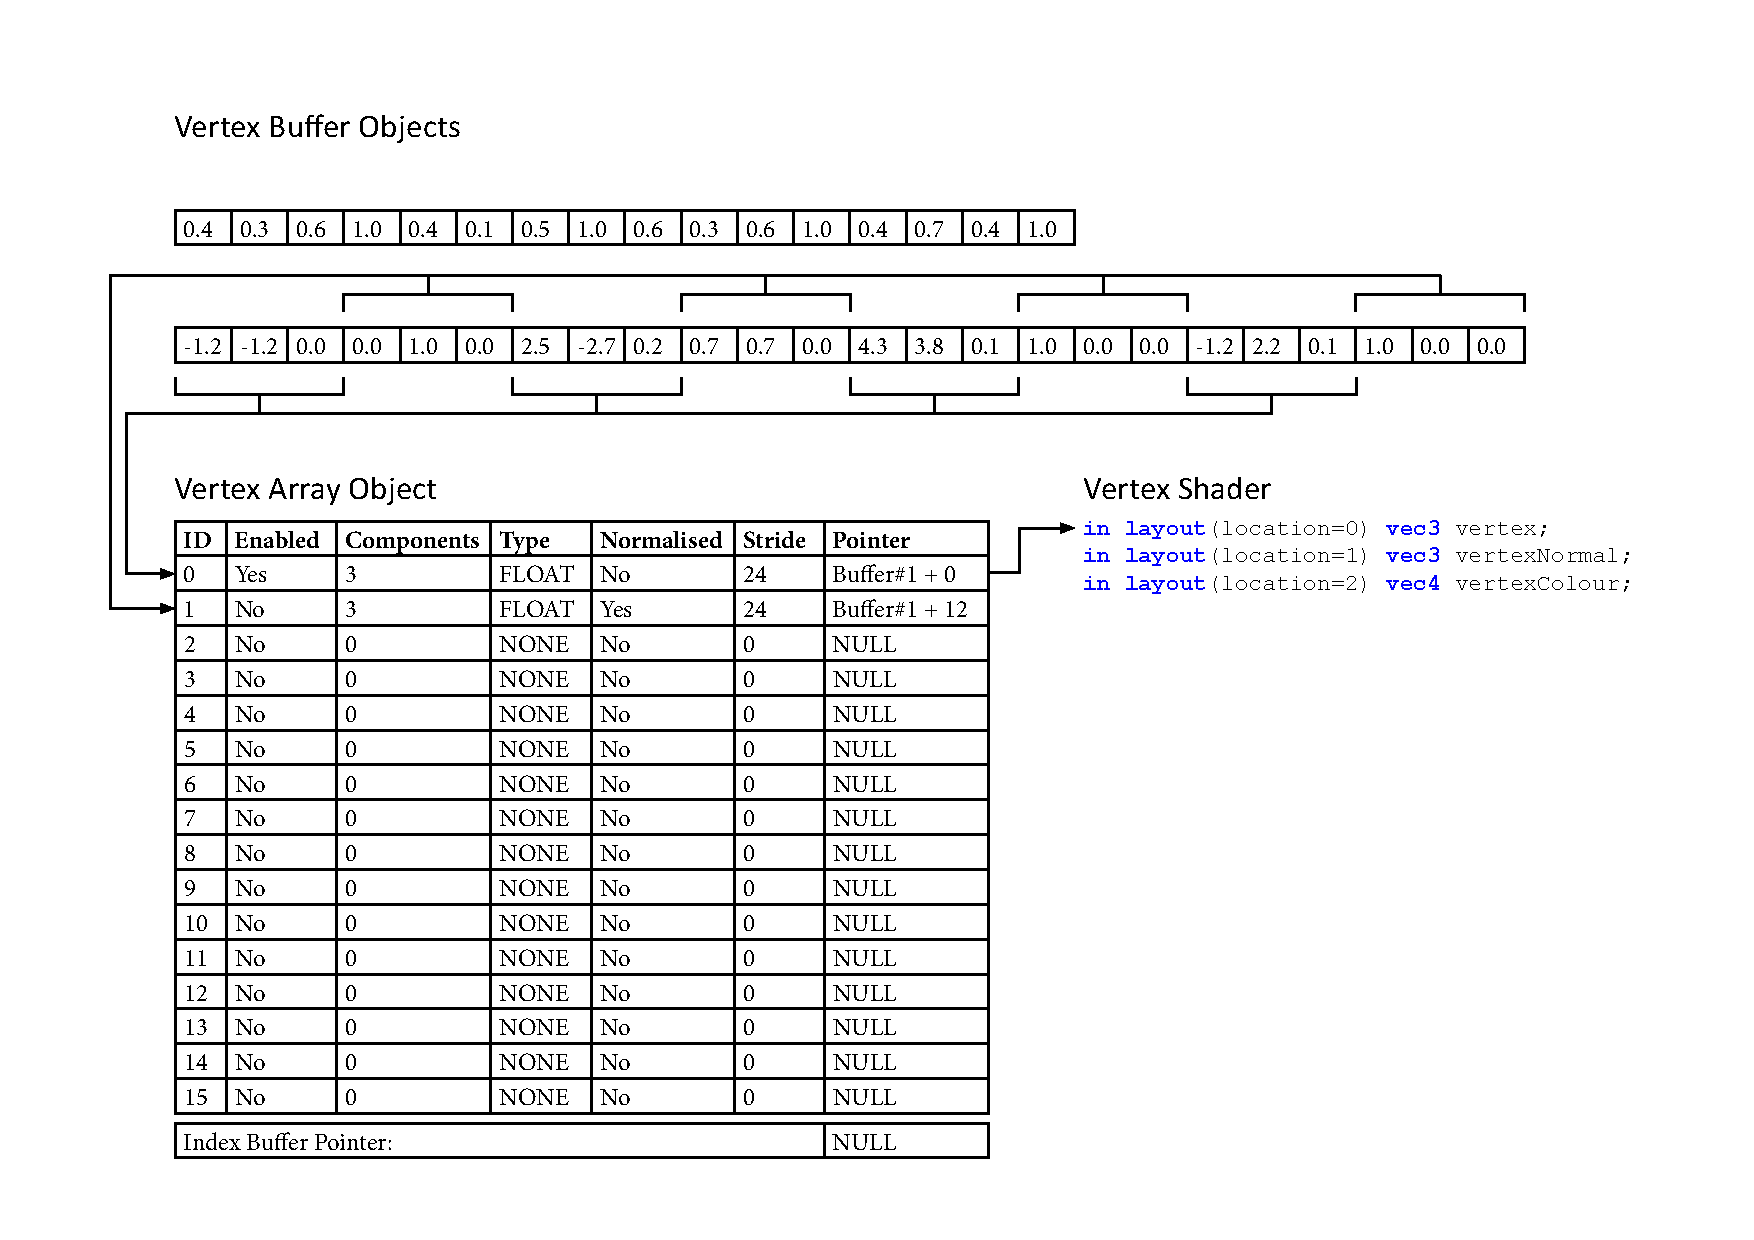
\includegraphics[width=210mm]{images/VAO_norm.pdf}}

The story is fairly similar as for the first vertex attribute. The only difference here is that the input data for the vertex normals start at a later point in the VBO. As you can see, there's a vertex coordinate which precedes it. 

This is a situation where the starting byte of the buffer needs to be adjusted. To do so, you can use the final parameter of the \mintinline{c}{glVertexAttribPointer()}. In this case, there are 3 floats of 4 bytes each preceding the first byte of the vertex normals attribute. This yields a starting byte of 12, which has been indicated separately in the VAO table.

However, the starting byte does not affect the stride, which is the same for both cases.

In the case of vertex normals, which by definition ought to be normalised, it is possible to enable normalisation using a parameter of the \mintinline{c}{glVertexAttribPointer()} function. In this example it has mainly been enabled for the sake of showing a situation where it could be useful, though in practice it's not always a necessity.

\newpage

\makebox[\textwidth]{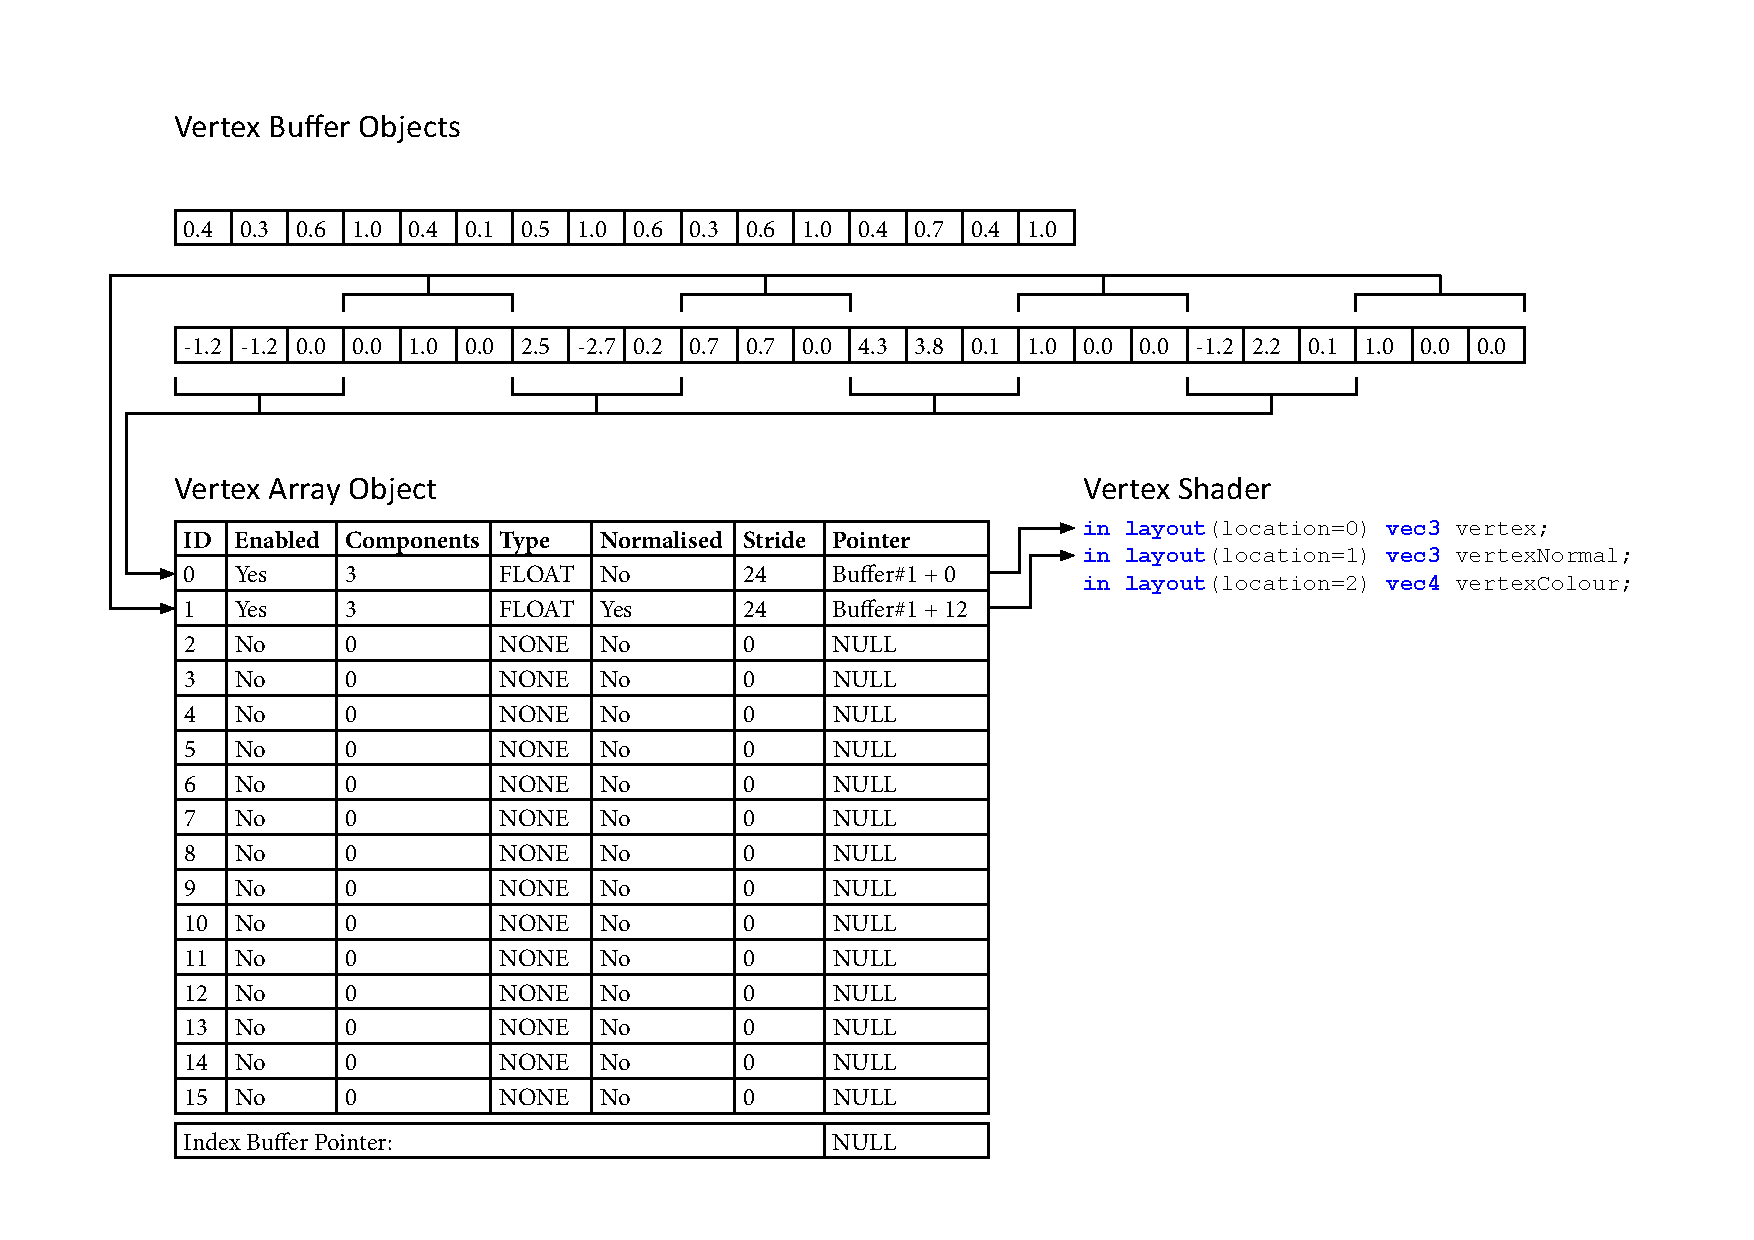
\includegraphics[width=210mm]{images/VAO_norm_enabled.pdf}}

Again we call \mintinline{c}{glEnableVertexAttribArray()} to create a connection between the VAO entry and the shader input. Note that unlike the VBO's there's no connection created between the VAO and a shader. Instead, think of it as ``opening the floodgates'' to allow input values to flow from the VBO's to a shader input. 

Not calling \mintinline{c}{glEnableVertexAttribArray()} will therefore prevent any inputs from reaching their respective shader input.

\newpage

\makebox[\textwidth]{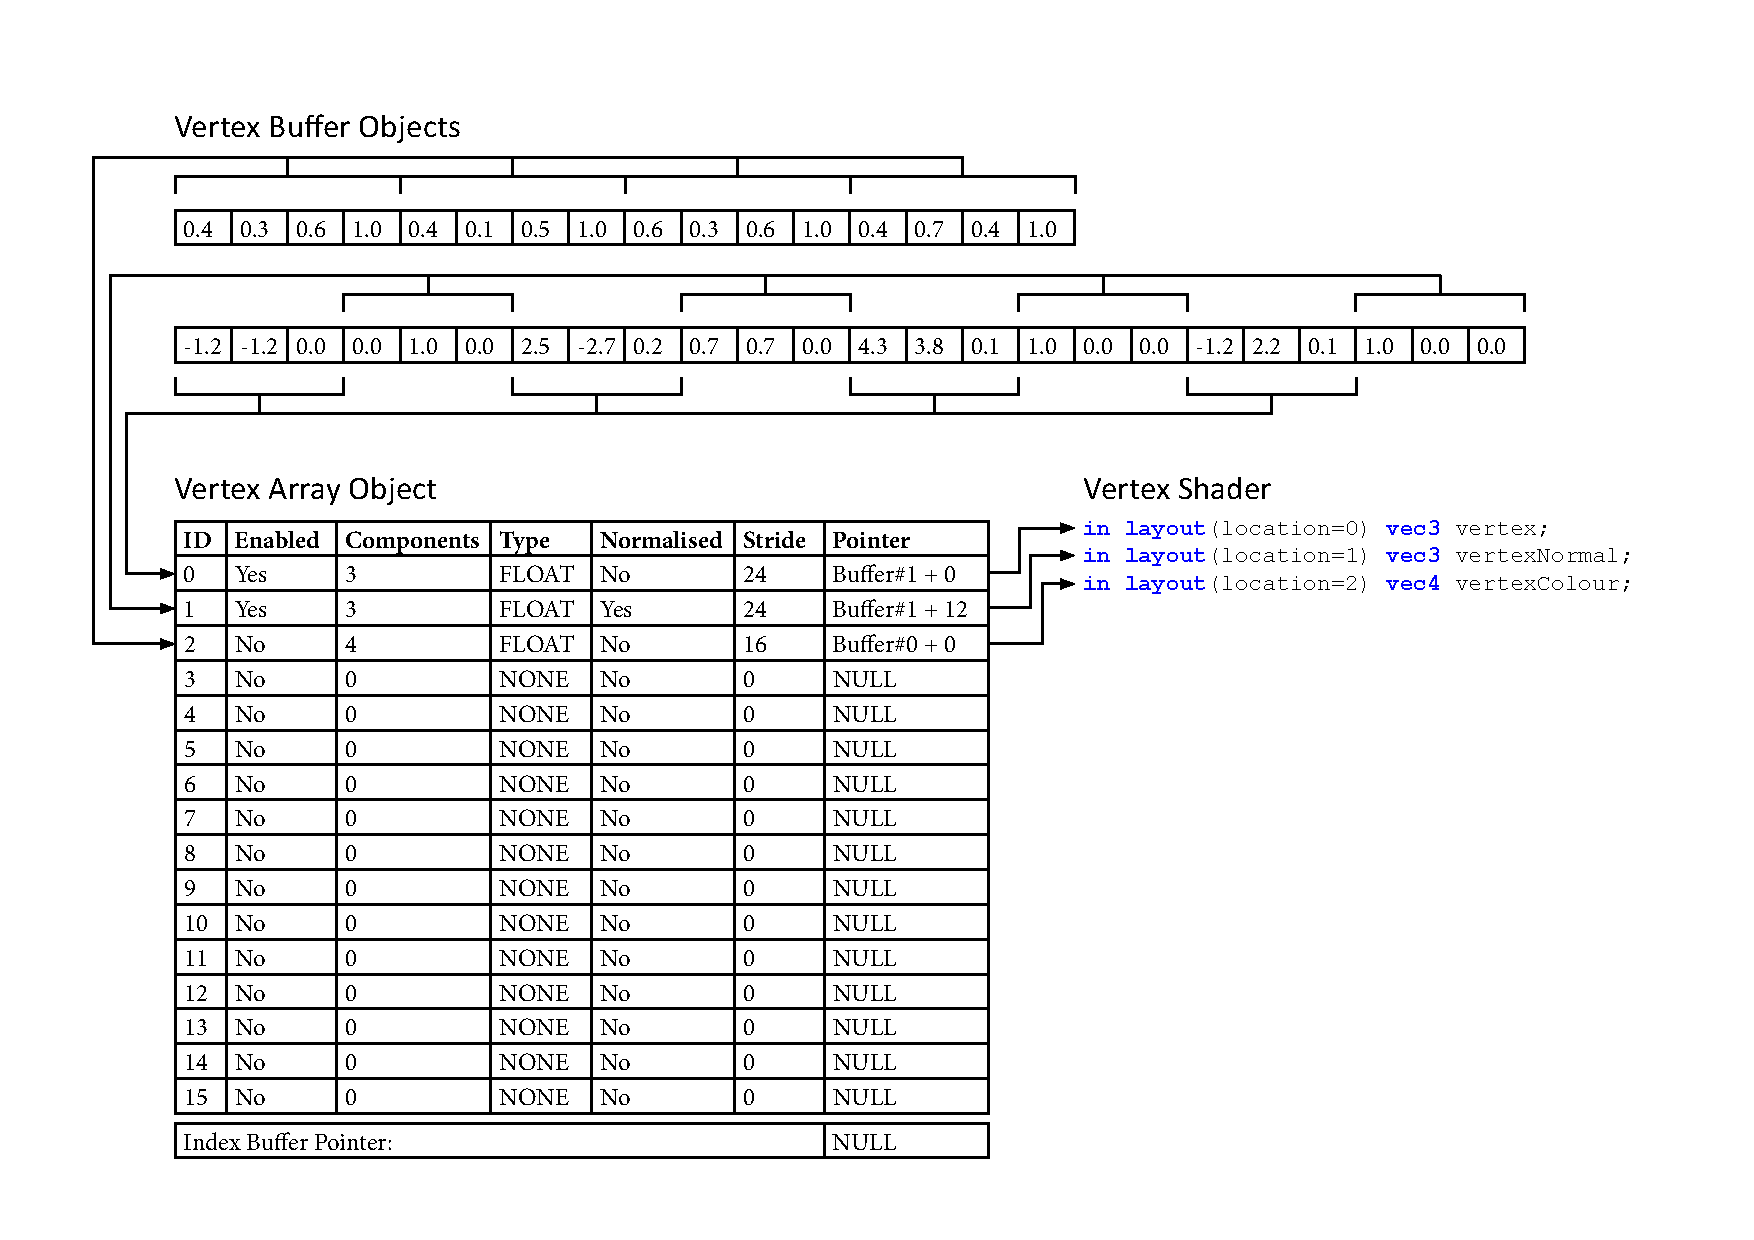
\includegraphics[width=210mm]{images/VAO_colour.pdf}}

Here's one more attribute for good measure. There are a few things different with this one. First, the data for this vertex attribute originates from a different VBO. Again, this assumes ``buffer\#0'' was bound while calling \mintinline{c}{glVertexAttribPointer()}. 

Second, this buffer object has 4 elements per entry rather than 3. This results in there being 4 entries * 4 bytes per entry = 16 bytes between the start of each subsequent entry, which is the stride. 

\newpage

\makebox[\textwidth]{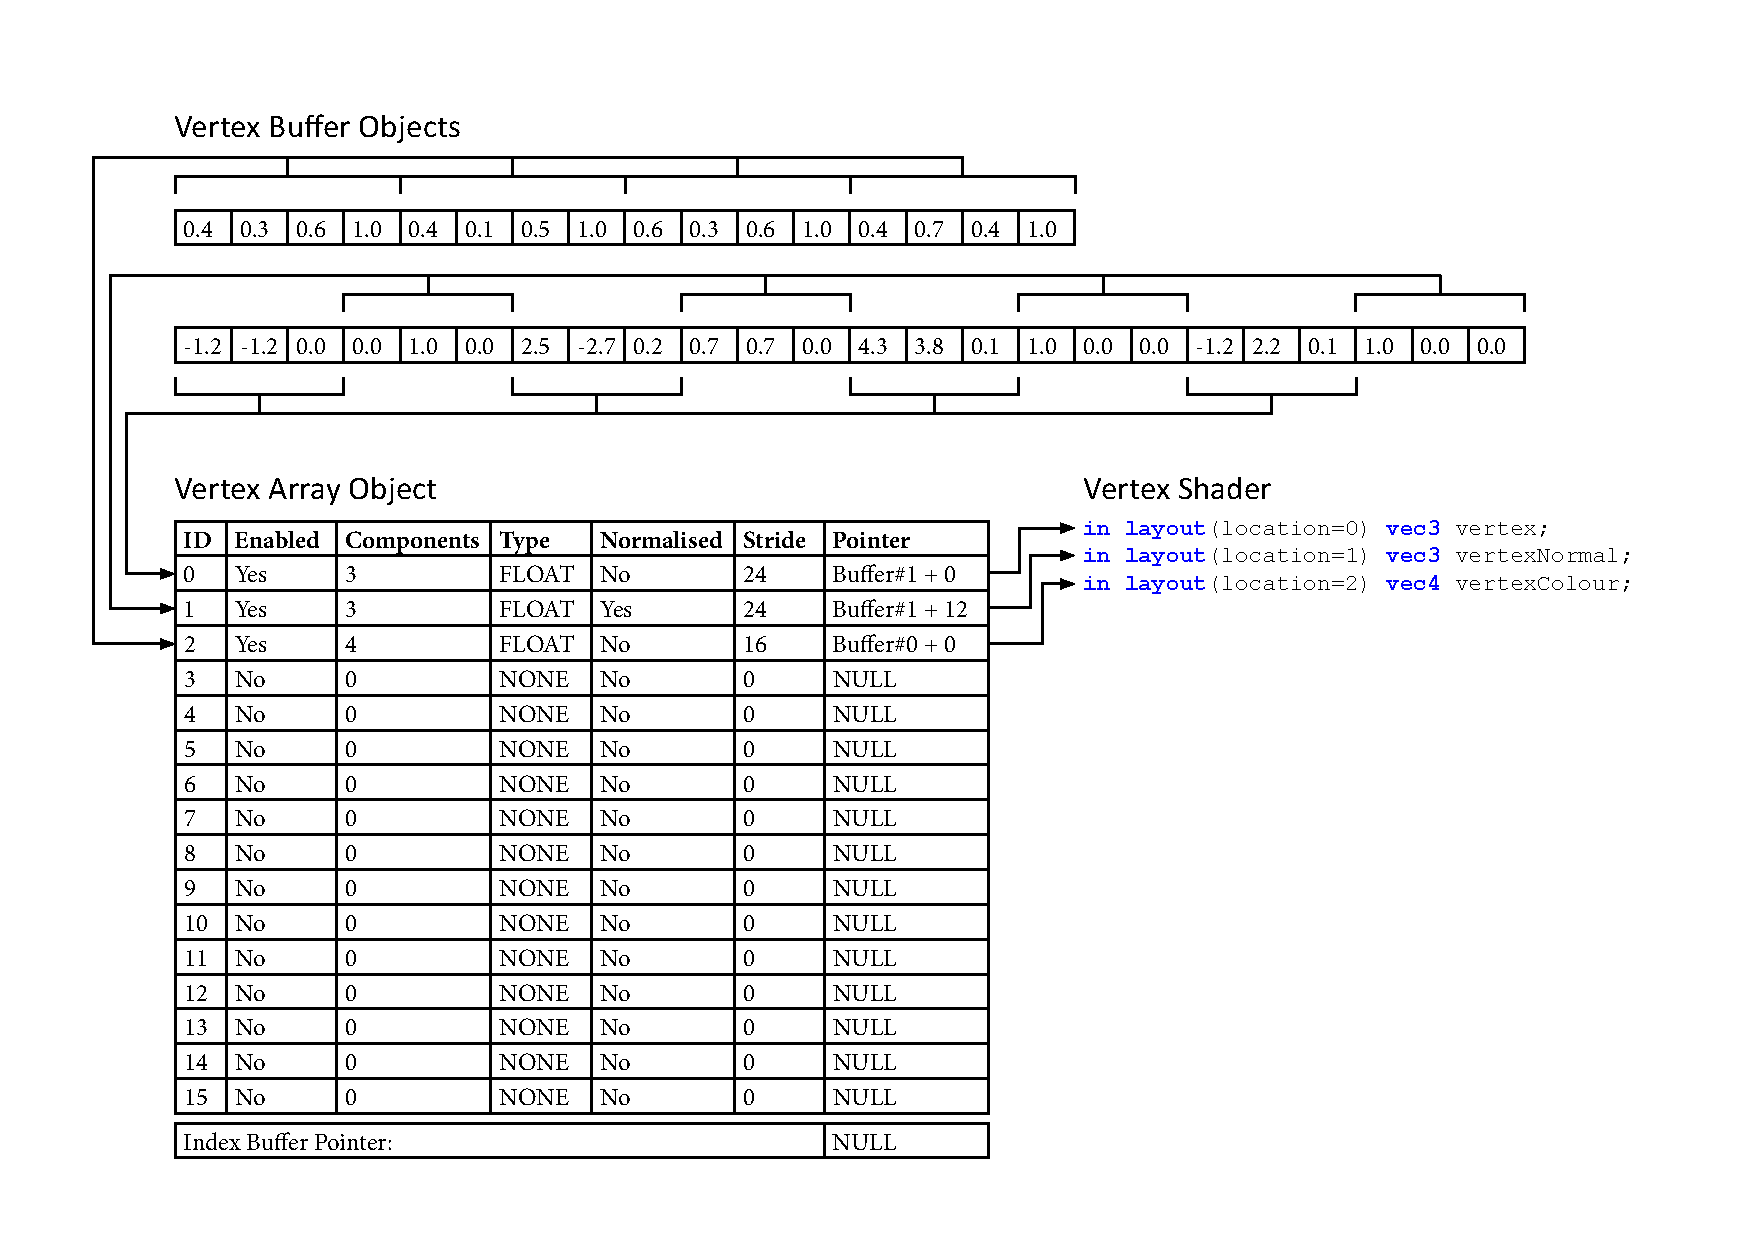
\includegraphics[width=210mm]{images/VAO_colour_enabled.pdf}}

And finally we enable the attribute using a call to \mintinline{c}{glEnableVertexAttribArray()}. Hopefully you have gotten the idea at this point.

\section{Drawing Vertex Array Objects}

\subsection{Overview}

So where have we gotten up to this point? Here's a diagram showing the buffers we set up:

\centerline{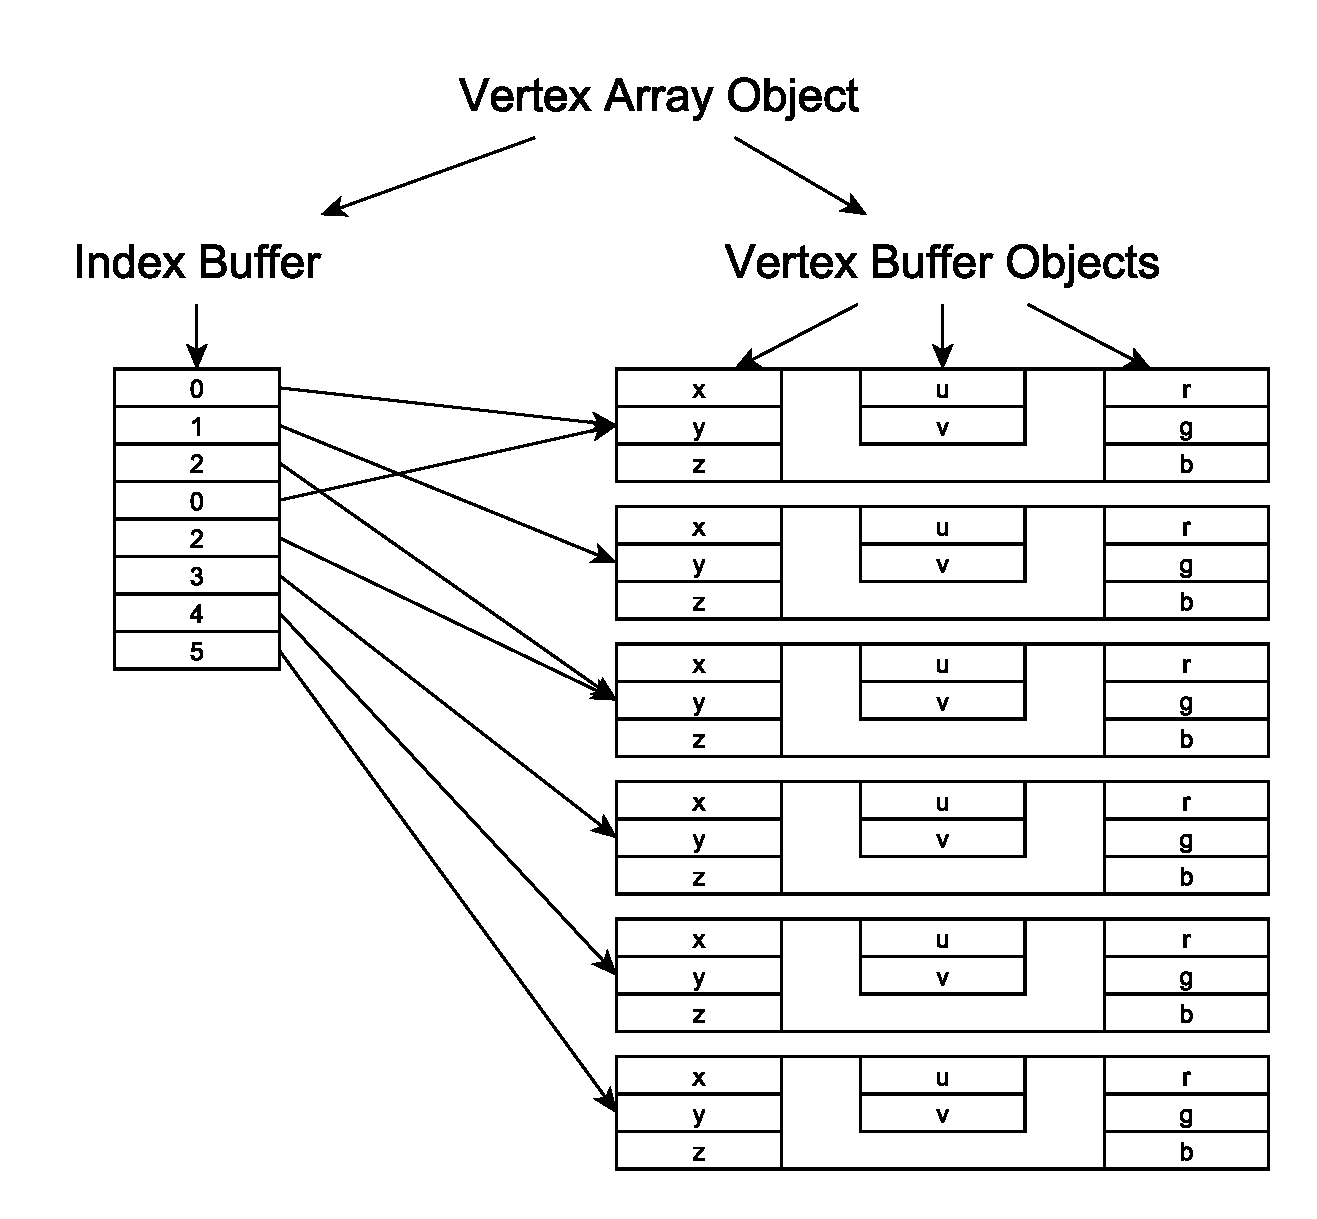
\includegraphics[scale=0.6]{images/openGL_index_buffer.eps}}

We have created a Vertex Array Object which consists of reference to an Index Buffer and references to one or more Vertex Buffer Objects. The Vertex Array Object also contains Vertex Attribute specifications, which a vertex shader can take as input. All a vertex shader needs to do at this point is specify which input should draw its data from which Vertex Attribute.

We will now see how to initiate this rendering process. Don't worry, it's a lot simpler than setting up the VAO!

\subsection{Drawing the Vertex Array Object}

As the frame buffer has to be cleared every frame (the handout code already contains a call to \mintinline{c}{glClear()}), you have to redraw the scene every single frame. Drawing a scene usually happens in a loop known as the ``main loop''. The handout code already has one set up for you. You can insert your drawing calls in there.

The first step of drawing a VAO is to bind it. This works exactly the same way as when we set it up; a single call to \mintinline{c}{glBindVertexArray()}. After this, any drawing command will use this VAO as input. You can only draw from a single VAO at a time.

\subsubsection{Issuing the draw command}

As we have already set up the VAO in its entirety previously, OpenGL already knows how to interpret the various Vertex Buffer Objects, and which Vertex Attributes they will provide. As such we just have to call a single function to draw the VAO:

\begin{minted}{c}
void glDrawElements(enum mode, int count, enum type, void* indices);
\end{minted}

\mintinline{c}{glDrawElements} will cause a draw call to be issued, and use the Vertex Attributes specified in the VAO as input to the rendering pipeline. 

The \mintinline{c}{mode} parameter specifies the type of primitive you'd like to draw. The basic primitive modes are \mintinline{c}{GL_POINTS}, \mintinline{c}{GL_LINES} and \mintinline{c}{GL_TRIANGLES}.

Here are some other handy drawing modes that combine the basic primitives:
\begin{description}
\item[\mintinline{c}{GL_LINE_STRIP}] \hfill \\
		Start with one vertex. For every vertex that follows, draw a line from the previous vertex to the current one.
\item[\mintinline{c}{GL_LINE_LOOP}] \hfill \\
		Same as \mintinline{c}{GL_LINE_STRIP}, but adds an additional line from the last to the first vertex.
\item[\mintinline{c}{GL_TRIANGLE_STRIP}] \hfill \\
		Works similar to a line strip, but uses the previous 2 vertices and the current vertex as coordinates of the triangle. 
\item[\mintinline{c}{GL_TRIANGLE_FAN}] \hfill \\
		Handy for drawing circles. Start with a centre vertex and a vertex on the edge of the circle. Every vertex you add draws a triangle through the centre vertex, the previous and the current one.
\end{description}

The \mintinline{c}{count} parameter specifies how many elements from the index buffer should be drawn. Note that this is the \emph{number of elements}, not the \emph{number of triangles, lines or points}. For example, in the case of \mintinline{c}{GL_TRIANGLES}, \mintinline{c}{count} should always be a multiple of 3.

\mintinline{c}{Type} specifies the data type of the values in your index buffer. This is usually \mintinline{c}{GL_UNSIGNED_INT}, although \mintinline{c}{GL_UNSIGNED_SHORT} and \mintinline{c}{GL_UNSIGNED_BYTE} are also accepted if you happened to specify your indices using those data types.

Finally, \mintinline{c}{indices} specifies the start index in your index buffer to start drawing from. Just pass in 0 here.

Unfortunately, we're not quite ready yet to draw your VAO. As mentioned previously, the rendering pipeline by default is missing a vertex and fragment shader. We'll need to specify those before we can send any draw calls through the pipeline.
\chapter{Introduction to GLSL}

\section{Shaders in OpenGL}

We've seen in the previous section how geometry can be specified and how a draw call can be issued in OpenGL. Now we address two other important issues in rendering images: where does the object appear in the scene, and what colour(s) does it have? Oh, and how do we ensure an image comes out of the pipeline in the first place?

All of these are accomplished through something known as a \emph{Shader}. In OpenGL, a Shader is a small program that runs on the GPU. Usually shaders are run once in their entirety for every single input item they process. In the case of a vertex shader, this would be vertices. There exist a number of types of Shaders for different purposes. 

Shaders are commonly invoked many times (in the order of millions) to render even a single frame. There's a range of different kinds of Shaders, but most of them are irrelevant unless you're trying to do something very advanced.

In practice, you'll commonly only be using two particular types of Shaders:

\begin{itemize}
  \item The Vertex Shader
  \item The Fragment Shader
\end{itemize}

As we've seen before, these shaders form an integral part of the rendering pipeline, and we're required to specify them before issuing any draw calls. For reference, here's the diagram showing the pipeline we've seen in chapter 1. Note where the Vertex and Fragment shaders are located in the pipeline.

\centerline {
	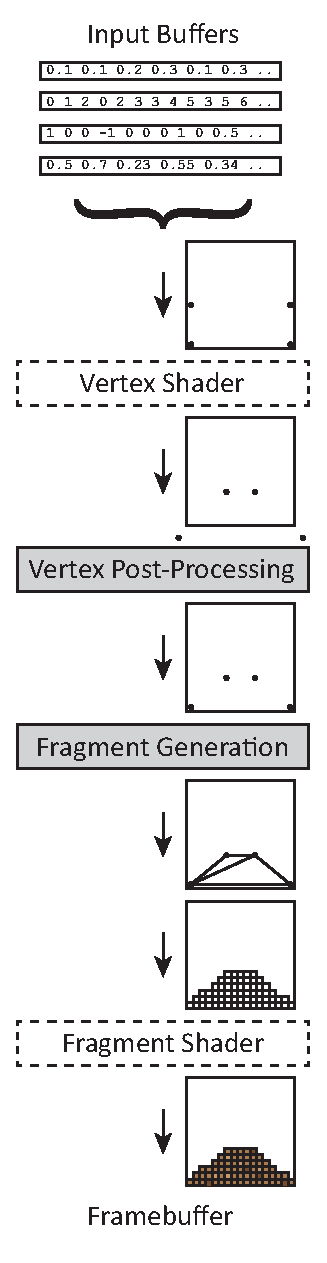
\includegraphics[scale=1.1]{images/pipeline-overview.eps}
}

The Vertex Shader runs once for every single vertex that is drawn. It is responsible for transforming (translating, scaling, rotating, etc.) individual vertices around the scene. This is for instance used to move objects around the scene, or to place them in desired locations. 

Additionally, the Vertex Shader is responsible for projecting the scene on to the camera. Projections are used to define how the world looks through the \emph{lens} of the camera. For example, a ``perspective projection'' causes objects that are further away from the camera to shrink in size, mimicking the way the human eye perceives a scene. Here is the effect of a perspective projection on a scene with two spheres:

\begin{figure}[htbp]
  \centering
  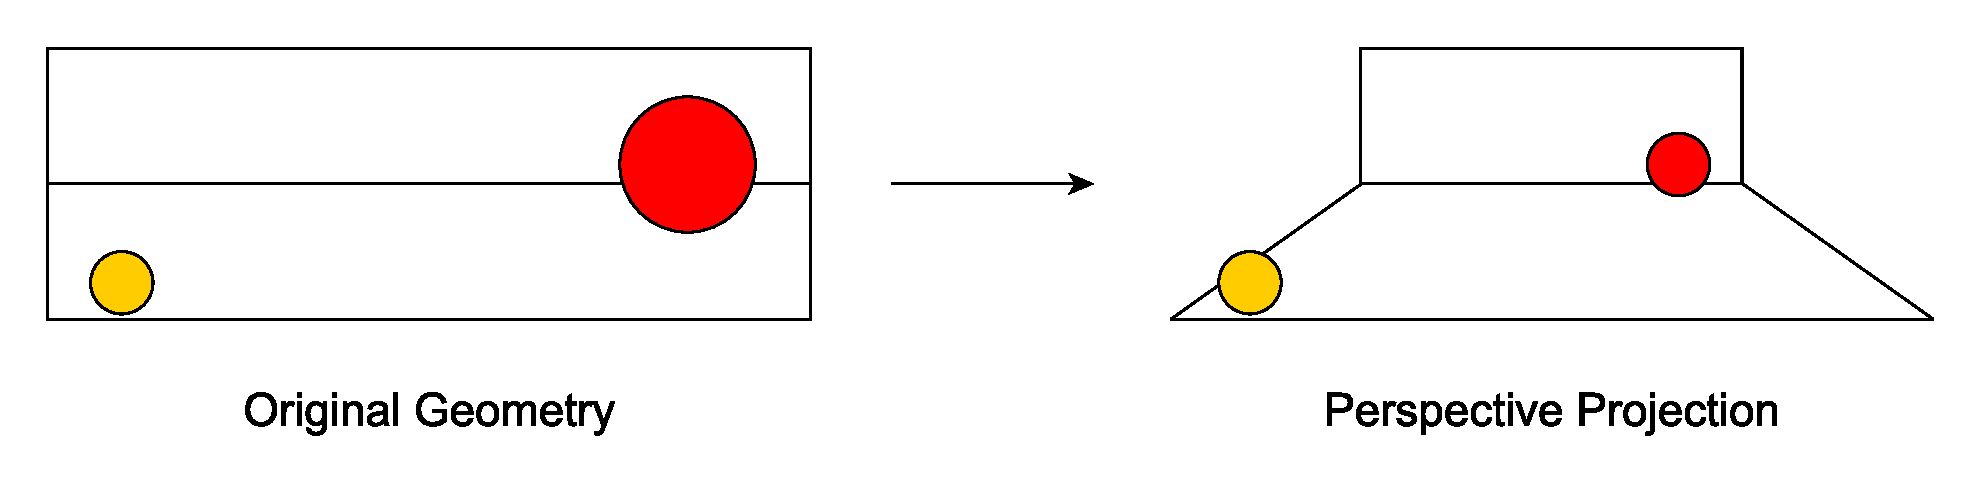
\includegraphics[scale=0.45]{images/openGL_perspective_projection.eps}
\end{figure}

After the Vertex Shader has finished processing all vertices, OpenGL uses the geometry specification to figure out which geometric primitives it should draw. These can either be points, lines or triangles. It then rasterises these primitives into pixels.

This is where the Fragment Shader comes in, which is responsible for determining the colour of each fragment. Fragments are pixels OpenGL attempts to draw. These may end up behind other geometry, thus not being visible in the final frame. They are thus not exactly the same thing as pixels on screen \footnote{The Direct3D equivalent of the Fragment Shader is called the ``Pixel Shader''. I suppose Microsoft ultimately calls it what it is, while OpenGL makes a distinction.}.

The Fragment Shader is executed once for {\bf every single} fragment. For complicated scenes this may imply rendering significantly more fragments than there are pixels on the screen.

\section{The GLSL Language}

So how exactly does one write a Shader? The OpenGL standard describes a language, imaginatively called the ``OpenGL Shading Language'', or GLSL for short.

GLSL is designed as a dialect of C, with a number of additions and limitations. We will therefore mainly look at the differences between these two languages. However, due to the extensive number of features in GLSL not all language components will be mentioned here for the sake of simplicity. As such you should not consider this overview complete or exhaustive, but it should include everything you need to complete the assignments.

\newpage

\subsection{General Layout of a Shader}

A minimal Shader source file commonly follows a specific layout. This layout has been outlined below:

\begin{minted}{glsl}
#version xxx
// Line 1: GLSL version declaration (this *HAS* to be line 1!)

// Input/output variable declaration
// For example: 
in layout(location=2) vec3 vertex;

// A main function
void main() {
	// Do things
}
\end{minted}

As you can see, there's a version declaration of which version of GLSL you are using, as well as a listing of what input values are required and returned by the Shader. Finally, the main function represents the entry point of the Shader. Note that unlike some versions of C, the main function in GLSL always returns \mintinline{glsl}{void}.

We'll take a look at each of these parts in the sections below.

\subsection{The \#version Statement}

The first line in every Shader {\bf must} be a declaration of which version of GLSL the Shader is written in. There have been a number of iterations of GLSL over the years, some of which have significantly changed the language syntax. 

We are using OpenGL 4.0 or higher in these labs, so the version statement should reflect that. For example, putting \mintinline{glsl}{#version 400} at the top of a shader file will cause OpenGL to use the revision of GLSL that accompanies OpenGL 4.0. If your graphics card can support it, I'd recommend using \mintinline{glsl}{#version 450} by default.

\subsection{The Input/Output Declaration}

Because the Vertex and Fragment Shaders are programmable stages of the OpenGL pipeline, they require input for their operation and are expected to produce certain kinds of output depending on their place in the pipeline. 

OpenGL requires these inputs and outputs to be defined as global variables in the Shader. To mark a variable as an input or output, you have to use the \mintinline{glsl}{in} and \mintinline{glsl}{out} keywords respectively, as shown below:

\begin{minted}{glsl}
in vec4 vertex;
out vec4 transformedVertex;
\end{minted}

Because OpenGL tries to be both helpful and versatile, the Vertex and Fragment Shader both require you to define different inputs and outputs. However, you can add inputs and outputs at will for your own purposes. Here's an overview of what you have to define in each case:

\begin{description}
  \item[Vertex Shader input:] \hfill \\
  You need to explicitly define input variables for any Vertex Attributes you specified in the VAO you'd like to render. Note that if you want to pass any additional attributes to the Fragment Shader, you also have to define those as inputs here, and assign them to the output variables in the Shader code. This will cause them to be passed on to the Fragment Shader.
  \item[Vertex Shader output:] \hfill \\ 
  You are required to somewhere in your Shader code set the predefined output variable \mintinline{glsl}{out vec4 gl_Position} containing the transformed location of the vertex being processed by the Shader. In addition, you can define additional outputs that will be passed on to the Fragment Shader in case additional values are required for calculating the colours of pixels.
  \item[Fragment Shader input:] \hfill \\
  Any values that have been explicitly passed on from the Vertex Shader. Note that because the Vertex Shader is only executed for every vertex instead of every pixel, values from different vertices are interpolated automatically by OpenGL before they are passed into the Fragment Shader.

  This can be turned off if desired (see the OpenGL documentation for details), but is in the vast majority of cases a useful feature.
  \item[Fragment Shader output:] \hfill \\ 
  Usually only a single \mintinline{glsl}{vec4} with RGBA format containing the colour of the fragment (pixel). Note that in GLSL all colour channel values range between 0 and 1. 
\end{description}

As mentioned previously, the VAO we specified contains vertex attribute with specific indices. The Vertex Shader must indicate which input variable should originate from which Vertex Attribute. 

OpenGL therefore contains a ``layout'' mechanism to identify these correspondences. If you look at the \mintinline{c}{glVertexAttribPointer()} function specification, the first parameter requires you to specify an index. To ensure that the correct Vertex Attribute is connected to the correct shader input, you just have to ensure that the index specified in \mintinline{c}{glVertexAttribPointer()} matches with the index of the shader input variable.

The easiest way for accomplishing this is to use the \mintinline{glsl}{layout(location=[index])} qualifier before your input declaration. For example, if we would like the input variable to correspond to a buffer with index 6, we can define the input variable as follows:

\begin{minted}{glsl}
in layout(location=6) vec4 vertex;
\end{minted}

If you want to pass on values to another Shader further down the pipeline, such as the Fragment Shader, you will also need to specify layout qualifiers, in the same way as you did for connecting vertex attributes to Shader inputs. You have to make sure that the output index of the Vertex Shader matches the input index of the Fragment Shader to ensure OpenGL understands this output and input correspond to each other. 

For illustration, the following output variable in the Vertex Shader:

\begin{minted}{glsl}
layout(location=2) out vec4 colour;
\end{minted}

Would correspond to this input variable in the Fragment Shader:

\begin{minted}{glsl}
layout(location=2) in vec4 thisNameCanBeDifferent;
\end{minted}

For reference, here's an overview over the entire pipeline:

\vspace{0.5cm}
\centerline {
  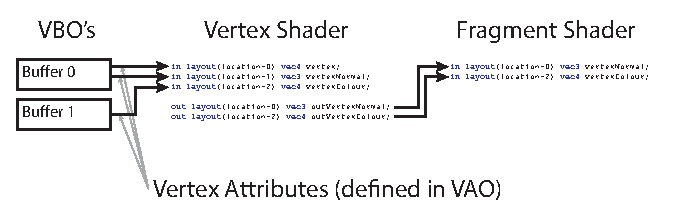
\includegraphics[scale=1.4]{images/overview.eps}
}
\vspace{0.5cm}

Note, however, that the layout qualifier feature is only available from OpenGL 4.3 or higher. If your graphics card and driver does not support this version, or you have configured Gloom to use an earlier version (it currently uses version 4.0 by default), you need to use a different method.

In this case there are two options.

First, it is possible to let OpenGL automatically determine the indices at which Vertex Attributes should be assigned. You can accomplish this by leaving out the location specification in the Shader source.

Next, ensure that your Shader is loaded and bound before you construct your VAO(s). You can now use the \mintinline{c}{glGetAttribLocation()} function to obtain the indexes which OpenGL has assigned to your inputs:

\begin{minted}{c}
int glGetAttribLocation(unsigned int programID, char* variableName);
\end{minted}

The first parameter is the ID of your Shader Program (these are explained in more detail in section \ref{sec:loadshader}), and the second is a string containing the name of the Shader's input variable. You should set the indexes passed in to \mintinline{c}{glVertexAttribPointer()} and \mintinline{c}{glEnableVertexAttribArray()} while setting up the VAO.

Alternatively, after compiling the shaders, but before linking them, it is possible to specify the input locations by calling the function \mintinline{c}{glBindAttribLocation()}. This function replaces the effect of layout specification syntax.

Of the two alternatives, this method is superior. However, it requires modification to the shader loading function supplied in Gloom. You can decide yourself which solution works best for you. All three methods are considered correct in the context of the grading of these labs.

\subsubsection{Uniforms}

There is another ``special'' kind of input to a Shader; the uniform variable. You can consider uniforms to be \emph{parameters} that are the same for every instance of your Shader that's being executed. Hence the name ``uniform''. 

You can use them to pass in a value of any type supported by GLSL into a Shader. They act as constants while the Shader is executing. You can thus only read from them from within the Shader itself. One application of uniforms is to define values that are the same throughout a single draw call, but still change from time to time. 

The value of a Uniform is kept between executions of the shader. It retains its value until it is changed. Note that this must always be done on the CPU side. Shader code is unable to change uniform values. Also note that GLSL considers uniforms inputs to your Shader. You should therefore specify positions for them explicitly, like you did with the inputs and outputs before. Here's an example: 

\begin{minted}{glsl}
uniform layout(location = 3) vec4 lightPosition;
\end{minted}

You can subsequently use the glUniform[number of elements][parameter datatype]() function to set the value(s) of the uniform. For the uniform defined above, this is how you can set its value in OpenGL:

\begin{minted}{c}
// Function used: 
// void glUniform4f(int index, 
//             float value1, float value2, float value3, float value4);
// Note that we above defined the location of the uniform to be 3
glUniform4f(3, 1f, 2f, 3f, 4f);
\end{minted}

If the layout specification syntax is not supported on your machine, you can use the \mintinline{c}{glGetUniformLocation()} function to obtain the index assigned to the input by OpenGL. An overview over the most relevant \mintinline{c}{glUniform()} function signatures is shown in table \ref{tab:uniforms}.

\begin{sidewaystable}
  \centering
\caption{A table showing the function signatures of the most commonly used flavours of glUniform().}
\label{tab:uniforms}
\begin{tabular}{|l|l|l|l|}
\hline
\textbf{Input Data Type} & \textbf{C Data Type} & \textbf{GLSL Data Type} & \textbf{Function Signature} \\ \hline
float & \begin{tabular}[c]{@{}l@{}}float\\ glm::vec2\\ glm::vec3\\ glm::vec4\end{tabular} & \begin{tabular}[c]{@{}l@{}}float\\ vec2\\ vec3\\ vec4\end{tabular} & \begin{tabular}[c]{@{}l@{}}void glUniform1f(int location, float v0);\\ void glUniform2f(int location, float v0, float v1);\\ void glUniform3f(int location, float v0, float v1, float v2);\\ void glUniform4f(int location, float v0, float v1, float v2, float v3);\end{tabular} \\ \hline
int & \begin{tabular}[c]{@{}l@{}}int\\ glm::int2\\ glm::int3\\ glm::int4\end{tabular} & \begin{tabular}[c]{@{}l@{}}int\\ int2\\ int3\\ int4\end{tabular} & \begin{tabular}[c]{@{}l@{}}void glUniform1i(int location, int v0);\\ void glUniform2i(int location, int v0, int v1);\\ void glUniform3i(int location, int v0, int v1, int v2);\\ void glUniform4i(int location, int v0, int v1, int v2, int v3);\end{tabular} \\ \hline
float matrix & \begin{tabular}[c]{@{}l@{}}glm::mat2x2\\ glm::mat3x3\\ glm::mat4x4\end{tabular} & \begin{tabular}[c]{@{}l@{}}mat2\\ mat3\\ mat4\end{tabular} & \begin{tabular}[c]{@{}l@{}}void glUniformMatrix2fv(int location, int count, bool transpose, float* value);\\ void glUniformMatrix3fv(int location, int count, bool transpose, float* value);\\ void glUniformMatrix4fv(int location, int count, bool transpose, float* value);\end{tabular} \\ \hline
\end{tabular}
\end{sidewaystable}

\subsection{Data Types}

There exist five basic datatypes in GLSL: \mintinline{glsl}{bool}, \mintinline{glsl}{int}, \mintinline{glsl}{uint}, \mintinline{glsl}{float} and \mintinline{glsl}{double}. Note that unlike C, integers are specified to be 32-bit values. Also, most modern graphics cards do not natively support double precision values, or are extremely slow at processing them (for a modern high-end card this can be a factor of 32 slower compared to single precision values). You'll therefore want to default to single precision whenever you need to work with floating point values, unless your \emph{really} need the precision.

GLSL also includes vector and matrix types for conveniently grouping data together. 

The most commonly used vector types are \mintinline{glsl}{vec2}, \mintinline{glsl}{vec3} and \mintinline{glsl}{vec4}, containing 2, 3 and 4 single precision floats respectively. You can create a new vector like this:
\begin{minted}{glsl}
vec4 vector = vec4(1.0, 0.0, 0.0, 1.0);
\end{minted}
And access individual elements like this:
\begin{minted}{glsl}
// method 1: use the built-in rgba components
float element0 = vector.r;
float element1 = vector.g;
float element2 = vector.b;
float element3 = vector.a;

// method 2: use the built-in xyzw components:
float element0 = vector.x;
float element1 = vector.y;
float element2 = vector.z;
float element3 = vector.w;

// method 3: use array indices:
float element0 = vector[0];
float element1 = vector[1];
float element2 = vector[2];
float element3 = vector[3];
\end{minted}

If you only need certain elements of the vector, you can also combine different properties like this:

\begin{minted}{glsl}
vec2 location2D = vector.xy;
vec3 colour = vector.rgb;
\end{minted}

Besides vectors, GLSL also contains built-in matrix types. These types are formatted as ``mat[number of columns]x[number of rows]''. For instance, the type of a matrix with 3 rows and 2 columns would be \mintinline{glsl}{mat2x3}. Unlike vector types, there is only one method for accessing matrices. 

Also note that matrices in OpenGL are column major. If you're not familiar with the term, column major means that you first address the column, then the row when dealing with multidimensional arrays, such as matrices. 

Here's a snippet of code showing how to use them:

\begin{minted}{glsl}
// defines the matrix: [1, 2]
//                     [3, 4]
mat2x2 matrix = {{1, 3}, {2, 4}};
// changes it to: [1, 2]
//                [5, 4]
matrix[0][1] = 5.0;
\end{minted}

%Finally, if you would like to use textures in your Shader, you have to pass their ID into the Shader as a uniform variable. The type of this uniform will not be an integer, but a \mintinline{glsl}{sampler2D}. If you want to sample a pixel in your texture, you have to use the \mintinline{glsl}{texture()} function. Here's how to use it:

%\begin{minted}{glsl}
%in layout(location = 4) sampler2D sampler;

%void main() {
%    // Texture coordinates are usually defined by the geometry specification.
%    // So in practice you usually get these from the Vertex Shader.
%    vec2 textureCoordinates = vec2(0.5, 0.5);
%    vec4 texturePixelColour = texture(sampler, textureCoordinates);
%}
%\end{minted}

\subsection{Operators}

Even though most operators such as addition, subtraction or multiplication work exactly the same as in C, there are some notable differences with GLSL.

First of all, you can't typecast in GLSL in the way you can in C. Instead, you can in most cases call the type you want to convert to as a ``function''. Here's an example showing how to convert from a float to an int:

\begin{minted}{glsl}
int intValue = int(floatValue);
\end{minted}

Secondly, you can use the basic arithmetic operators (+, -, *, /) on matrices and vectors, or a combination of the two. Do note that this follows the rules of matrix multiplication. So addition performs element wise addition, given that the matrices or vectors are of equal dimensions.

Here's some examples:
\begin{minted}{glsl}
// Creates a 4x4 matrix with 1's in the leading diagonal; 
// the identity matrix.
mat4x4 matrix = mat4(1); 

vec3 positionXYZ = vec3(1, 2, 3);
vec4 positionXYZW = vec4(1, 2, 3, 1);

// Compilation error: a 4x4 matrix can't be multiplied with a 3x1 matrix
vec4 error = matrix * positionXYZ; 

// returns vec4(1, 2, 3, 1) as anything multiplied with the 
// identity matrix results in the same matrix.
vec4 newPosition = matrix * positionXYZW; 

// returns vec3(2, 4, 6)
vec3 doublePosition = 2 * positionXYZ; 
\end{minted}


\subsection{Language Constructs}

The remainder of GLSL should pretty much be downhill from here on out, because it's practically the same as C :)

But let's go over them for the sake of reference.

First of all, the if statement. You really want to avoid these as much as possible, as the branch instructions generated by if statements are incredibly expensive on GPUs. Especially considering that the Vertex and Fragment Shaders are executed many times per frame.

Moreover, modern GPUs tend to cluster cores together in order to allow them to share part of the processor logic. This for instance includes instruction decoding. It allows the size of each individual core to be shrunk, and as a result more cores can fit on the die.

This also affects the way shaders are executed. Specifically, if a branch instruction causes some cores to choose the \emph{if} clause and some the \emph{else} clause, \emph{both} clauses are executed. Cores which chose the \emph{else} clause will need to wait until the \emph{if} clause is finished, and vice versa. As such you don't get a speedup in the execution of your shader the way you would if it were executed on a CPU. It may even cause a slowdown.

\begin{minted}{glsl}
if(someVariable > 3) {
	// Do something
} else {
	// Do something else.
}
\end{minted}

The same is true for for loops. If you need the performance, it's usually better to look for alternate strategies or redundancies to avoid having to use branching.

\begin{minted}{glsl}
for(int i = 0; i < 10; i++) {
	// Do something
}
\end{minted}

That also counts for the while loop:

\begin{minted}{glsl}
while(someCondition != false) {
	// Do something
}
\end{minted}

And finally, you can define additional functions if you need them:

\begin{minted}{glsl}
bool isGreaterThan(float a, float b) {
	return a > b;
}
\end{minted}

\section{Loading and using Shaders}
\label{sec:loadshader}

You've hopefully gotten a sense at this point on how to write a Shader. Now we should take a look at how to set them up and use them. 

In terms of the lab work, doing this yourself is not required, though if you want to implement the procedure yourself you're welcome to do so. An implementation of the shader loading procedure has been implemented for you in the file Shader.hpp.

As opposed to Direct3D's shader model, OpenGL has opted for a local compilation approach. This means that whenever you want to use a shader on the user's machine, you have to compile it locally. Major graphics card vendors therefore include GLSL compilers in their graphics drivers.

This may sound like an odd decision at first. After all, why do you not compile it once on your development machine, and save everyone else the effort? 

The problem is that modern graphics hardware differs from vendor to vendor. The binary code generated by each vendor's compiler may differ significantly. Local compilation avoids tricky situations where you have to compile explicitly for each vendor's card, possibly even different models. Local compilation is therefore a more fitting approach. 

\subsection{The Shader Program Object}

In OpenGL shaders are grouped together into so-called \emph{Program Objects}. The idea is that each shader is compiled individually, attached to a Program Object and finally linked together. Once set up, Program Objects can be activated at will.

The linking stage is responsible for checking that shader combinations are compatible. That is, that one shader's output specifications match with another shader's input specification.

The resulting structure looks something like this:

\centerline {
  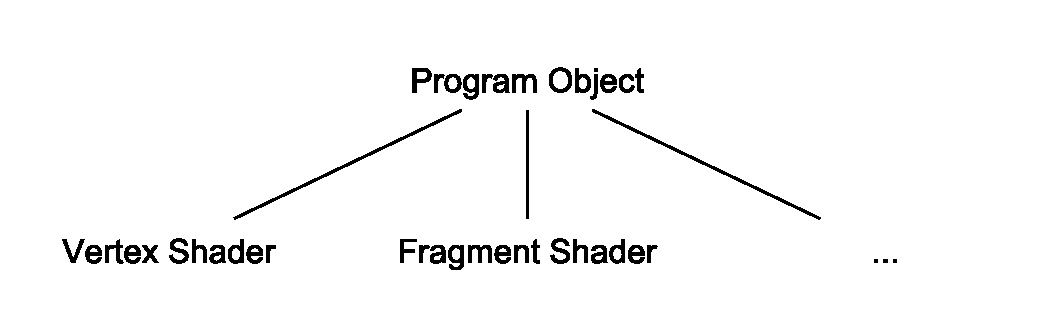
\includegraphics[scale=0.6]{images/openGL_program_structure.eps}
}

First off, we create a new Program Object using:

\begin{minted}{c}
unsigned int glCreateProgram();
\end{minted}

Once again, the function does not return a structure or object, but an ID that can be used to refer to the object in OpenGL calls.

\subsection{Loading and Compiling a Shader}

Next, we need to load and compile each of the shaders we would like to use. OpenGL does not provide any means for loading shader source code from a file, so loading a text file into memory is your responsibility. 

Hint: it may be useful to drop the loading of a single shader in its own function as the process is nearly identical for each shader type.

Compiling a shader starts with the creation of a Shader object:

\begin{minted}{c}
unsigned int glCreateShader(enum shaderType);
\end{minted}

The shaderType parameter specifies the type of shader you are creating. Some relevant options are:

\begin{itemize}
  \item \mintinline{c}{GL_VERTEX_SHADER}
  \item \mintinline{c}{GL_FRAGMENT_SHADER}
\end{itemize}

Next we pass in the source code of the shader Program using:

\begin{minted}{c}
void glShaderSource(
        unsigned int shaderID, 
        int count, 
        char** strings, 
        int** lengths
);
\end{minted}

The \mintinline{c}{shaderID} parameter is the ID returned by \mintinline{c}{glCreateShader()}.

The source string itself can either be one large string, or chopped up into smaller bits. Appending them all together should give the complete source code of the Shader.

\mintinline{c}{Count} represents the number of parts you have divided the Shader source code into. \mintinline{c}{Strings} and \mintinline{c}{lengths} are arrays of strings and integers, respectively. \mintinline{c}{Strings} contains the actual source code, and \mintinline{c}{lengths} the length of each string in \mintinline{c}{strings}. 

Now that the source code is in place, we can compile it using:

\begin{minted}{c}
void glCompileShader(unsigned int shaderID);
\end{minted}

Although you're strictly not required to, it's very good practice to check for compilation errors. 

You can check whether compiler errors occurred using:

\begin{minted}{c}
int shaderCompilationStatus = 0;

// glGetShaderiv() allows requesting information about a shader.
// In this case the compilation status (GL_TRUE if success, GL_FALSE if not)
glGetShaderiv(shaderID, GL_COMPILE_STATUS, &shaderCompilationStatus);

bool compilationErrorsOccurred = shaderCompilationStatus == GL_FALSE;
\end{minted}

If an error occurred, you can obtain an information log using:

\begin{minted}{c}
int logLength = 0;

// Again using glGetShaderiv() for obtaining the log length
glGetShaderiv(shaderID, GL_INFO_LOG_LENGTH, &logLength);

// Allocating enough memory to store the info log
char* infoLog = (char*) malloc(logLength);

glGetShaderInfoLog(shaderID, logLength, NULL, infoLog);

// Print the info log:
printf("A Shader compilation error occurred. Info log:\n");
printf("%s\n", infoLog);

free(infoLog);
\end{minted}

You can delete a shader to free up memory if the shader is not going to be used for a significant stretch of time. You can do so using:

\begin{minted}{c}
void glDeleteShader(unsigned int shaderID);
\end{minted}

And we're done! Run this process for both the Vertex and Fragment shaders, and we can move on to the linking stage of compilation.

\subsection{Attaching and Linking Shaders}

After compiling both shaders, you have to attach each shader to the Program object you created. The \mintinline{c}{glAttachShader()} function does just that:

\begin{minted}{c}
void glAttachShader(unsigned int programID, unsigned int shaderID);
\end{minted}

This will make Shaders a part of the Program Object. 

Now that all shaders have been attached to the Program Object, we can perform the linking stage of compilation:

\begin{minted}{c}
void glLinkProgram(unsigned int programID);
\end{minted}

Again, it is strictly not necessary to check for linking errors, but doing so is considered good practice. The process is almost identical compared to Shader compilation error checking. You can obtain the linking status of your Program by calling:

\begin{minted}{c}
int programLinkStatus = 0;

glGetProgramiv(programID, GL_LINK_STATUS, &programLinkStatus);
bool linkingFailed = programLinkStatus == GL_FALSE;
\end{minted}

Obtaining the error log is also the same compared to Shaders, apart from the OpenGL function calls:

\begin{minted}{c}
int logLength = 0;

// Using glGetProgramiv() instead of glGetSDhaderiv().
// The functions have the same intent; obtaining information
// about the Program and Shader, respectively.
glGetProgramiv(programID, GL_INFO_LOG_LENGTH, &logLength);

// Allocating enough memory to store the info log
char* infoLog = (char*) malloc(logLength);

glGetProgramInfoLog(shaderID, logLength, NULL, infoLog);

// Print the info log:
printf("Program linking failed. Info log:\n");
printf("%s\n", infoLog);

free(infoLog);
\end{minted}

And that's it. We can now use the Program object at will. When enabled, the Shaders you defined will take their respective places in the OpenGL pipeline, and do whatever you have instructed them to do.

\subsection{Enabling and Disabling the Program Object}

The only thing that now remains is the question of how to activate your Program Object. This can be done by calling:

\begin{minted}{c}
void glUseProgram(unsigned int programID);
\end{minted}

Passing in your programID will activate it. Passing in 0 will restore OpenGL's default behaviour.

\subsection{Debugging Shaders}

Because shaders are executed in such large quantities and communication between the CPU and GPU is complicated, it is very difficult to debug one. The Fragment Shader is in my own experience the most complicated one to get right, so I tend to use the fragment colour as a debug value. 

For instance, if a value becomes inexplicably large, you can insert an if statement that checks for such large values. It can then set the pixel colour to red, which makes it visible to you.

Another tip is to read your shader's source code. Shader code tends to (and should!) be very short. The problem space is therefore usually much smaller than typical CPU code. Careful reading can therefore get you quite far.

Some graphics card vendors supply debug tools for their card which you can also give a try.

\newpage

\begin{center}
	\vspace{9cm}
	\resizebox{\linewidth}{!}{\textbf{Don't Panic}}
\end{center}

\end{document}
